\documentclass{article}
\usepackage{graphicx} 
\usepackage{float}
\usepackage{booktabs}
\usepackage{array}
\usepackage{arydshln}
\usepackage{siunitx}
\usepackage{hyperref}
\usepackage{cancel}
\usepackage{changepage}
\usepackage{placeins}
\usepackage{enumitem}
\usepackage{siunitx}
\usepackage{lipsum}
\usepackage[most]{tcolorbox}


%\usepackage{showframe}
\usepackage{times}

\DeclareSIUnit{\atm}{atm}

\usepackage{tabularx}
\usepackage{amsmath, amssymb, amscd, MnSymbol, mathrsfs}
\usepackage{cellspace}
\usepackage{tikz}
\usetikzlibrary{calc,3d, patterns, angles, quotes, decorations.markings, decorations.pathmorphing, hobby}
\usepackage{xfrac}

\usepackage{chemfig}
\usepackage{caption}
\usepackage{bm}
\usepackage{pdfpages}
\usepackage{empheq}
\usepackage{pgfplots}
\usepackage{pgfplotstable}
\usepackage{xstring}

\pgfplotsset{compat=1.18}
\usepackage[oldvoltagedirection]{circuitikz}
\usepackage{microtype}
\usepackage{tikz-3dplot}
\usepackage{textcomp}
% Custom commands
\newcommand{\vect}[1]{\boldsymbol{\mathbf{#1}}}
\newcolumntype{C}{>{\centering\arraybackslash}X}
\newcolumntype{M}[1]{>{\centering\arraybackslash}m{#1}}

\usetikzlibrary{external}
\tikzexternalize[prefix=figures/]

\newcommand\myfrac[2]{\sfrac{#1\mkern-1.2mu}{#2}}
\usepackage{xcolor}

% Define custom colors
\definecolor{darkblue}{rgb}{0.1,0.1,0.5} % A dark blue shade
\definecolor{formalshade}{rgb}{0.95,0.95,1} % A light blue shade for the background

% For the adjustwidth environment
\PassOptionsToPackage{strict}{changepage}
\usepackage{changepage}

% For formal definitions
\usepackage{framed}

\newcommand{\formalsource}{} % Initialize an empty macro to store the source text

\newenvironment{formal}[3][]{% Start of the environment
	\renewcommand{\formalsource}{#1}% Store the optional argument
	\def\FrameCommand{%
		\hspace{1pt}%
		{\color{#2}\vrule width 2pt}%
		{\color{#3}\vrule width 4pt}%
		\colorbox{#3}%
	}%
	\MakeFramed{\advance\hsize-\width\FrameRestore}%
	\noindent\hspace{-4.55pt}% Disable indenting the first paragraph
	\begin{adjustwidth}{}{7pt}%
		\vspace{2pt}%
	}%
	{%
		\vspace{4pt}%
		\ifx\formalsource\empty % Check if the source is empty
		\else
		\hfill{\footnotesize{\formalsource}}% Align source to the bottom-right
		\fi
	\end{adjustwidth}\endMakeFramed%
}


% Custom itemize list with images for positive and negative items
\newlist{gitemize}{itemize}{1} % Just one level for the list
\setlist[gitemize,1]{
	leftmargin=2.8em, % Adjust the margin for the list
	labelsep=1em % Control the space between the label and the list item
}

% Define checkmark and cross symbols for positive and negative items
\newcommand{\checkitem}{\raisebox{-0.25\height}{\includegraphics[width=0.4cm]{checkmark.png}}}
\newcommand{\crossitem}{\raisebox{-0.25\height}{\includegraphics[width=0.4cm]{cross.png}}}


\usepackage[left=0.8in,right=0.8in,top=0.5in,bottom=0.69in,includeheadfoot,letterpaper]{geometry}
\usepackage{fancyhdr}
\usepackage{graphicx}
\usepackage{tabularray}
\usepackage{varwidth} 


\newcommand{\wm}[2]{%
	\begin{minipage}{#1\textwidth}
		\centering
		#2
	\end{minipage}%
}

\pagestyle{fancy}
\fancyhf{}


\renewcommand{\headrulewidth}{0.4pt}
\renewcommand{\footrulewidth}{0.4pt}

\fancyhead[L]{\includegraphics[height=1.2cm]{images/Kingston_University_London_logo_200-tablet.png}}
\fancyhead[R]{EG4024 – ME – Fluid Mechanics and Thermodynamics}
\fancyfoot[C]{Department of Mechanical Engineering}
\fancyfoot[R]{\thepage}

\usepackage{scalerel}

\setlength{\headheight}{30pt}
\setlength{\footskip}{20pt}



\usepackage[export]{adjustbox}
\usepackage{tocloft}
\renewcommand{\cfttoctitlefont}{}
\renewcommand{\contentsname}{}
\renewcommand{\cftsecleader}{\cftdotfill{\cftdotsep}}

\setlength{\cftbeforesecskip}{0.5em}



\usepackage{hyperref}    % For hyperlinks
\usepackage{xurl}        % For better URL handling
\hypersetup{
	colorlinks=true,
	linkcolor=blue!50!black,
	urlcolor=blue,       % Color for URLs
}


\definecolor{ChineseGold}{HTML}{C59401}
\definecolor{AmericanGold}{HTML}{D3AF37}
\definecolor{MetallicSunburst}{HTML}{A77C37}
\definecolor{GoldenBrown}{HTML}{996515}
\definecolor{DarkBrown}{HTML}{674222}
\definecolor{SkyBlue}{HTML}{87CEEB}      % Soft and bright
\definecolor{BabyBlue}{HTML}{89CFF0}     % Gentle, pastel-like
\definecolor{SteelBlue}{HTML}{4682B4}    % Rich but not overpowering
\definecolor{RoyalBlue}{HTML}{4169E1}    % Strong, slightly purplish
\definecolor{MidnightBlue}{HTML}{191970} % Almost black, deep navy
\definecolor{PrussianBlue}{HTML}{003153} % Very deep blue with a classic look


\usepackage{listings}

\definecolor{codegreen}{rgb}{0,0.6,0}
\definecolor{codegray}{rgb}{0.5,0.5,0.5}
\definecolor{codepurple}{rgb}{0.58,0,0.82}
\definecolor{backcolour}{rgb}{0.95,0.95,0.92}

\lstdefinestyle{mystyle}{
	backgroundcolor=\color{backcolour},   
	commentstyle=\color{codegreen},
	keywordstyle=\color{magenta},
	numberstyle=\tiny\color{codegray},
	stringstyle=\color{orange},
	basicstyle=\ttfamily\scriptsize,
	breakatwhitespace=false,         
	breaklines=true,                 
	captionpos=b,                    
	keepspaces=true,                 
	numbers=left,                    
	numbersep=5pt,                  
	showspaces=false,                
	showstringspaces=false,
	showtabs=false,                  
	tabsize=2
}

\lstset{style=mystyle}

%Refer to the equation as \eqref{equation}.
\usepackage{caption}  % This package allows captioning outside of a float
\usepackage[export]{adjustbox}


\usetikzlibrary{patterns}

\usetikzlibrary{patterns.meta}
\usepackage[para]{footmisc} % Example of making footnotes run together in a paragraph

\definecolor{darkgreen}{rgb}{0.0, 0.5, 0.0}

\usepackage{datetime}

\usepackage{etoolbox}

\makeatletter
\def\tagform@#1{\maketag@@@{{Eq.~#1}}} 
\makeatother

\usepackage{ifthen}
\usepackage{calc}
\usepackage{datenumber}

\usepackage{physics}
\usepackage[outline]{contour}
\usetikzlibrary{patterns,decorations.pathmorphing}
\usetikzlibrary{arrows.meta}
\tikzset{>=latex}
\contourlength{1.1pt}

\colorlet{mydarkblue}{blue!50!black}
\colorlet{myred}{red!65!black}
\colorlet{watercol}{blue!80!cyan!10!white}
\colorlet{darkwatercol}{blue!80!cyan!20!white}
\tikzstyle{piston}=[blue!50!black,top color=blue!30,bottom color=blue!50,middle color=blue!20,shading angle=0]
\tikzstyle{water}=[draw=mydarkblue,top color=watercol!90,bottom color=watercol!90!black,shading angle=5]
\tikzstyle{vertical water}=[water,
top color=watercol!90!black!90,bottom color=watercol!90!black!90,middle color=watercol!80,shading angle=90]
\def\tick#1#2{\draw[thick] (#1)++(#2:0.1) --++ (#2-180:0.2)}


% Initialize counters
\newcounter{deadlineyear}\setcounter{deadlineyear}{2025}
\newcounter{deadlinemonth}\setcounter{deadlinemonth}{4}
\newcounter{deadlineday}\setcounter{deadlineday}{3}
\newcounter{mydatenumber}  % Date conversion
\newcounter{currentdate}   % Current date
\newcounter{daysdiff}      % Days difference
\newcounter{currenttime}   % Current minutes since midnight
\newcounter{totalminutes}  % Total remaining minutes
\newcounter{displaydays}   % Days to display
\newcounter{remainingmins} % Remaining minutes after days
\newcounter{displayhours}  % Hours to display
\newcounter{displaymins}   % Minutes to display

% Main calculation command
\newcommand{\timeUntilDeadline}{%
	% Calculate days between dates
	\setmydatenumber{mydatenumber}{\thedeadlineyear}{\thedeadlinemonth}{\thedeadlineday}%
	\setmydatenumber{currentdate}{\the\year}{\the\month}{\the\day}%
	\setcounter{daysdiff}{\themydatenumber - \thecurrentdate}%
	
	% Get current time in minutes since midnight
	\setcounter{currenttime}{\time}%
	
	% Calculate total remaining minutes
	\setcounter{totalminutes}{\numexpr\thedaysdiff * 1440 - \thecurrenttime}%
	
	% Check deadline status
	\ifnum\thetotalminutes < 0
	\textbf{\color{red}Deadline passed!}%
	\else
	% Calculate time components
	\setcounter{displaydays}{\thetotalminutes / 1440}%
	\setcounter{remainingmins}{\numexpr\thetotalminutes - \thedisplaydays * 1440}%
	\setcounter{displayhours}{\theremainingmins / 60}%
	\setcounter{displaymins}{\numexpr\theremainingmins - \thedisplayhours * 60}%
	
	% Format output
	\textbf{%
		\ifnum\thedisplaydays > 0
		\thedisplaydays\ day\ifnum\thedisplaydays > 1 s\fi%
		\ifnum\thedisplayhours > 0
		\ifnum\thedisplaymins > 0, \else\ and \fi%
		\else
		\ifnum\thedisplaymins > 0\ and \fi%
		\fi%
		\fi%
		\ifnum\thedisplayhours > 0
		\thedisplayhours\ hour\ifnum\thedisplayhours > 1 s\fi%
		\ifnum\thedisplaymins > 0\ and \fi%
		\fi%
		\ifnum\thedisplaymins > 0
		\thedisplaymins\ minute\ifnum\thedisplaymins > 1 s\fi%
		\fi%
		\ left}%
	\fi
}

\definecolor{mygreen}{HTML}{07a56d}

\newtcbtheorem{briefillus}{Definiton}{
	enhanced,
	sharp corners,
	attach boxed title to top left={
		xshift=0pt, 
		yshift=-\tcboxedtitleheight, 
		yshifttext=-\tcboxedtitleheight/2-0.5em
	},
	colback=white,
	colframe=black,
	fonttitle=\bfseries,
	coltitle=white,
	boxed title style={
		rounded corners,
		arc=2pt,
		size=small,
		colback=black,
		colframe=black,
	},
	leftrule=0pt, 
	rightrule=0pt, 
}{thm}



\newcounter{dataset}

% 2. Create a custom environment
\newenvironment{datasetbox}[2]{
	\refstepcounter{dataset}
	\begin{tcolorbox}[
		title={\color{black}\textbf{Dataset \thedataset: #1}},
		colback=black!4!white,
		colframe=black!10!white,
		boxrule=0.5mm,
		width=\textwidth,
		label={#2}]
	}{\end{tcolorbox}}



\begin{document}
	
	\vspace*{\fill}
	\begin{center}
		\textbf{\Huge Laboratory Report}\\[10pt]
		\LARGE \textbf{Pressure}
	\end{center}
	\vspace*{\fill}
	
	\Large    
	\begin{tabular}{@{}l l l@{}}
		\textbf{Submitted by:} & Sakariye Abiikar (Group Leader) & K2371673 \\
		& Alireza Alishahi & K2333243 \\
		& Naim Alrifai & K2459662 \\
		& Munachi J Atuegbu & K2463699 \\
		& Ehsan Haque & K2453799 \\
		& Abdul Mueed & K2454880 \\   
		& Abdelrahman Shehata & K2426523 \\   
		& Varley, Freddie & K2311322
	\end{tabular}
	
	\vspace*{\fill}
	
	\begin{tabular}{@{}l l@{}}
		\textbf{Key Dates:} & Date of practical: Wednesday 19$^{\text{th}}$ March, 2025 \\
		& Deadline: Tuesday 3$^{\text{rd}}$ April, 2025 \\
		& Last Updated: \today\, \currenttime\\
		& Days left until deadline: \timeUntilDeadline \\
	\end{tabular}
	\vspace*{\fill}
	
	\large
	\newpage\noindent	\vspace*{-1em}
	
	\begin{center}
		\LARGE \textbf{Contribution Table}\\[2em]
	\end{center}	
	
	
	\begin{tblr}{
			colspec={Q[4cm]Q[4cm]Q[4cm]Q[3cm]},
			hlines,vlines,
			cells={valign=m,halign=c},
			rows={ht=4\baselineskip},
			row{1}={ht=1.5\baselineskip,font=\bfseries},
			row{Z}={bg=black!10!white},
			row{8}={bg=red!10!white}
		}
		Student & Course & Contribution & Picture \\ 
		Sakariye Abiikar & Mechanical Engineering & Formatter, Method \& Experimental Procedures, Introduction, Results & \includegraphics[width=2cm,valign=c]{images/image(7).jpeg} \\ 
		Alireza Alishahi & Mechanical Engineering  & Abstract, Method \& Experimental Procedures & \includegraphics[width=2cm,valign=c]{images/8_orgid_297f9608-cce6-40e3-adc2-86e161e7141f.jpg} \\ 
		Varley, Freddie & Mechanical Engineering & Theory, Recommendations &  \includegraphics[width=2cm,valign=c]{images/profile.png}\\
		Abdul Mueed & Mechanical Engineering  & \wm{0.1}{Theory\\ \small in progress} & \includegraphics[width=2cm,valign=c]{images/profile.png} \\ 
		Abdelrahman Shehata & Mechanical Engineering  & \wm{0.2}{Discussion of results\\ \small in progress} & \includegraphics[width=2cm,valign=c]{images/Image.jpg}\\
		Naim Alrifai & Mechanical Engineering & \wm{0.1}{Conclusion\\ \small in progress} & \includegraphics[width=2cm,valign=c]{images/Image(9).jpeg} \\\hline
		Munachi J Atuegbu & Mechanical Engineering & No contact at all might not be real. Last seen 11/29/24 is crazy & \includegraphics[width=2cm,valign=c]{images/profile.png} \\\hline
		Ehsan Haque & Mechanical Engineering & Approved Mitigation  & \includegraphics[width=2cm,valign=c]{images/profile.png} \\
	\end{tblr}
		\vspace*{\fill}
	
	\normalsize
	\newpage\newgeometry{top=0.2in,bottom=0.6in,left=0.8in,right=0.8in}
	\noindent\vspace{0em}
	\begin{center}
		\LARGE \textbf{Table of Contents}\\[-7em]
	\end{center}
	{
		\hypersetup{linkcolor=black}
		\tableofcontents
	}    
	
	
	\large\newpage\restoregeometry\vspace*{-20pt}
	
	\noindent
	
\section{Abstract}
In this experiment, we calibrated and compared the performance of multiple pressure-measuring devices, including two Bourdon gauges, a Budenberg pressure gauge and a Hg glass manometer, in tandem with a reference pressure calibrator (DPI-603 Portable Pressure Calibrator), which served as the baseline for pressure measurements and as the source of the applied pressure. The devices were connected to the DPI-603 Portable Pressure Calibrator, enabling us to apply both positive and negative pressures in increments of approximately 5 kPa. Through this process, we were able to get an exhaustive dataset that demonstrated notable differences in the pressure-measuring devices' performance. \textcolor{red!50!white}{[Placeholder breif results findings]}. These results highlighted the importance of selecting appropriate devices based on precision requirements and operating conditions, as well as the potential impact of human error in reading analog instruments like the Bourdon gauges and Hg manometer. 

	
	\newpage\vspace*{-20pt}

	\section{Introduction}
	In engineering and scientific applications, pressure measurement is essential, playing a critical role in fields such as fluid dynamics, meteorology, and industrial control. Over time, pressure-measuring instruments have evolved, from early liquid column manometers to modern mechanical and digital gauges, each designed to provide accurate measurements under varying conditions.\\[1em]
	A key distinction in pressure measurement is between \textbf{absolute} and \textbf{gauge} pressure.\\ 
	Absolute pressure is measured relative to a vacuum, while gauge pressure is measured relative to atmospheric pressure. This distinction influences the design and function of pressure-measuring devices.\\[1em]
	Historically, the invention of the Bourdon gauge by Eugène Bourdon in 1849 marked a significant advancement in pressure measurement. It provided a robust and reliable means of monitoring pressure in industrial settings, where durability and consistency were paramount. On the other hand, liquid column manometers, particularly those using mercury, have been essential in laboratory settings due to their precision in measuring small pressure differences.\\[1em]
	Despite the advantages of different pressure-measuring devices, each has limitations, such as calibration errors and environmental influences.\\[1em]
	Previous studies have highlighted various challenges and findings related to pressure measurement devices. For example, a study by Hodgkinson et al. (2020) found that the accuracy of home blood pressure monitors varied significantly, with validated monitors showing a higher pass rate in static pressure tests compared to unvalidated ones. This emphasizes the importance of validation and calibration in ensuring the accuracy of pressure-measuring devices.\\[1em]
	In this experiment, we aimed to evaluate the performance and accuracy of various pressure-measuring devices under controlled conditions, comparing their responses to varying pressure levels.
	
	\newpage\restoregeometry

	\section{Theory}

When we talk about pressure, the first thing that comes to mind is its physical definition. It refers to the effect or various types of deflection when a force is applied to a surface.\vspace{-0.5em}
\begin{center}
	\begin{minipage}{0.51\textwidth}
		\centering
			\begin{equation}
				P = \frac{F}{A}
				\label{eq:pressure}
			\end{equation}
		\hspace*{2em}\wm{0.9}{
			\begin{itemize}[itemsep=-1mm]
				\item \( P \) = Pressure (Pa, Pascal)
				\item \( F \) = Force applied (N, Newton)
				\item \( A \) = Surface area (m\(^2\))
			\end{itemize}
		}\\[9pt]\raggedright
		Local pressure \( P_{\text{local}}\) varies spatially. It peaks under concentrated loads (red zone) and vanishes at free edges (blue zone).\\[-1em]
		\begin{equation}
			P_{\text{local}} = \frac{dF}{dA}
			\label{eq:localpressure}
		\end{equation}	
		Critical for analyzing stress concentrations in engineering designs.
	\end{minipage}
	\hfill
	\begin{minipage}{0.46\textwidth}
		\vspace{-1.2em}\centering\hspace*{2.5em}
		\begin{tikzpicture}[scale=2,transform shape]
			\coordinate (c1) at (1,0,1);
			\coordinate (c2) at (-1,0,1);
			\coordinate (c3) at (-1,0,-1);
			\coordinate (c4) at (1,0,-1);
			\fill[blue!70!black,opacity=0.3] (c1) -- (c2) -- (c3) -- (c4) -- cycle;
			\begin{scope}
				\clip (c1) -- (c2) -- (c3) -- (c4) -- cycle;
				\begin{scope}[canvas is xz plane at y=0]
					\shade[inner color=red, outer color=blue!70!black, shading=radial,opacity=0.3] 
					(0,0) circle (1.36cm);
					\shade[inner color=red, outer color=blue!70!black!50!white, shading=radial, opacity=0.3] 
					(0,0) circle (1.2cm);
				\end{scope}
			\end{scope}
			\draw[thick] (c1) -- (c2) -- (c3) -- (c4) -- cycle;
			\draw[thick,-{Latex[scale=1.5,length=2mm,width=2mm]},line width=0.1mm] (0,1,0) node[above,right=1] {\large $\vec{F}$} -- (0,0,0);
			\draw[thick,<->] (1.05,-0.05,1.05) -- (-1.05,-0.05,1.05) node[midway,below=1.1] {\tiny$L_x$};
			\draw[thick,<->] (1.05,-0.05,1.05) -- (1.05,-0.05,-1.05) node[midway,right=1.1] {\tiny$L_x$};
			\node at (1.05,-0.05,1.05) [below] {$A$};
		\end{tikzpicture}
		\vspace{-1em}
		\captionof{figure}{Illustration of pressure application}
		\label{fig:pressure}\raggedright
		\vspace{1em}Average pressure $\left(P\right)$ assumes uniform distribution. Local pressure $\left(P_{local}\right)$ reveals real-world stress hotspots.
\end{minipage}\end{center}
Pressure measurement fundamentally relies on observing its physical effects on measurable systems. The accompanying figures demonstrate three classical approaches:\\[1em]
\begin{minipage}{1\textwidth}
\begin{minipage}{0.3\textwidth}\centering
\begin{tikzpicture}[scale=1.3,transform shape]
	\def\Rx{1.0}
	\def\Ry{0.05*\Rx}
	\def\rx{0.18*\Rx}
	\def\ry{0.06*\rx}
	\def\H{1.0}
	\def\h{0.72*\H}   % water level height
	\def\th{2.7*\H}   % tube height
	\def\ty{0.95*\th} % tube level
	\def\td{0.6*\h}   % tube depth
	\def\N{14}
	
	% WATER + CONTAINER
	\draw[vertical water] %rounded corners=2
	(-\Rx,\h) --++ (0,-\h) arc(180:360:{\Rx} and {\Ry}) --++ (0,\h);
	\draw[water]
	(0,\h) ellipse ({\Rx} and {\Ry});
	\draw[thick] (0,\H) ellipse ({\Rx} and {\Ry});
	
	% TUBE
	\draw[vertical water]
	(-\rx,\h) |-++ (2*\rx,\ty) --++ (0,-\ty);
	\draw[water]
	(0,\h+\ty) ellipse ({\rx} and {\ry});
	\draw[thick,line cap=round]
	(-\rx,\h) --++ (0,\th) coordinate (T) arc(180:0:\rx) --++ (0,-\th);
	\draw[mydarkblue,line cap=round]
	(-1.09*\rx,\h-0.005) arc(180:360:{1.09*\rx} and 1.12*\ry);
	\foreach \i [evaluate={\y=1.12*\H+0.84*\th*\i/\N}] in {0,...,\N}{
		\draw[line cap=round] (\rx,\y) arc(0:-50:{\rx} and \ry);
	}
	\begin{scope}
		\clip (-\Rx,\h) |-++ (2*\Rx,-\h) --++ (0,\h) arc(360:180:{\Rx} and {\Ry}) -- cycle;
		\draw[thick,line cap=round]
		(-\rx,\h) --++ (0,-\td) (\rx,\h) --++ (0,-\td);
		%(-\rx,\h) --++ (0,-\td) arc(180:360:{\rx} and {\ry}) --++ (0,\td);
		\draw[vertical water,opacity=0.5]
		(-\Rx,\h) --++ (0,-\h) arc(180:360:{\Rx} and {\Ry}) --++ (0,\h);
	\end{scope}
	\draw[mydarkblue]
	(-\Rx,\h) arc(180:360:{\Rx} and {\Ry});
	\draw[<->] (0.6*\Rx,\h) --++ (0,\ty) node[midway,fill=white,inner sep=1] {$h$};
	\draw[very thin,line cap=round]
	(T)++(130:\rx) node[anchor=-19,inner sep=1] {$P=0$} to[out=-50,in=170]++ (-30:1.5*\rx);
	\node[above] at (-0.6*\Rx,\H) {$P_\mathrm{atm}$};
	
	% CONTAINER
	\draw[thick]
	(-\Rx,\H) --++ (0,-\H) arc(180:360:{\Rx} and {\Ry})
	--++ (0,\H) arc(360:180:{\Rx} and {\Ry}) -- cycle;
	
\end{tikzpicture}
\captionof{figure}{Torricelli's method}
\end{minipage}\hfill
\vspace{1.5em}\begin{minipage}{0.3\textwidth}\centering\hspace*{-2.7em}
\begin{tikzpicture}[scale=1.4,transform shape]
	\def\W{0.8}       % pressure box height
	\def\H{0.7}       % pressure box height
	\def\Rx{0.55}     % tube bend radius horizontal
	\def\Ry{0.2*\Rx}  % tube bend radius vertical
	\def\rx{0.28*\Rx} % tube radius horizontal
	\def\ry{0.28*\Ry} % tube radius vertical
	\def\HL{1.3}      % tube height left
	\def\HR{2.2}      % stube height right
	\def\hL{0.40*\HL} % water level height left
	\def\hR{0.95*\HR} % water level height right
	%\def\th{2.7*\H}   % tube height
	%\def\ty{0.93*\th} % tube level
	\def\N{14}
	
	% WATER + CONTAINER
	\draw[water]
	(-\Rx,\hL) --++ (0,-\hL) arc(180:360:\Rx) --++ (0,\hR) --++ (2*\rx,0) --++
	(0,-\hR) arc(360:180:\Rx+2*\rx) --++ (0,\hL);
	\draw[water]
	(-\Rx-\rx,\hL) ellipse({\rx} and {\ry})
	(\Rx+\rx,\hR) ellipse({\rx} and {\ry});
	\draw[thick]
	(-\Rx,\HL) --++ (0,-\HL) arc(180:360:\Rx) --++ (0,\HR) coordinate (T) arc(180:0:\rx)
	--++ (0,-\HR) arc(360:180:\Rx+2*\rx) --++ (0,\HL);
	\draw[thick]
	(-\Rx-\rx,\HL) ellipse({\rx} and {\ry});
	\foreach \i [evaluate={\y=(\hL+\hR)/2+0.8*\HR*(\i-\N/2)/\N;}] in {0,...,\N}{
		\draw[line cap=round] (\Rx+2*\rx+0.007,\y) arc(0:-50:{\rx} and \ry);
	}
	%\draw[line cap=round,myred] (\Rx+2*\rx+0.007,{(\hL+\hR)/2}) arc(0:-70:{\rx} and \ry);
	\draw[line cap=round,myred] (-\Rx+0.007,\hL+\hR-\HR-\rx) arc(0:-70:{\rx} and \ry);
	\node at (-\W/2-2*\rx-\Rx,\HL+1.7*\rx) {$P_\mathrm{atm}$};
	\draw[very thin,line cap=round]
	(T)++(130:\rx) node[anchor=-19,inner sep=1] {$P=0$} to[out=-50,in=170]++ (-30:1.5*\rx);
	\draw[dashed] (-\Rx,\hL) --++ (1.3*\Rx,0) (\Rx,\hR) --++ (-1.3*\Rx,0);
	\draw[<->] (0,\hL) -- (0,\hR) node[midway,fill=white,inner sep=1] {$h$};
\end{tikzpicture}
\vspace{0.3em}
\captionof{figure}{Open manometers}
\end{minipage}\hfill
\begin{minipage}{0.3\textwidth}\centering\vspace{-0.9em}
\begin{tikzpicture}[scale=1.4,transform shape]
	\def\W{0.8}       % pressure box height
	\def\H{0.7}       % pressure box height
	\def\Rx{0.55}     % tube bend radius horizontal
	\def\Ry{0.2*\Rx}  % tube bend radius vertical
	\def\rx{0.28*\Rx} % tube radius horizontal
	\def\ry{0.28*\Ry} % tube radius vertical
	\def\HL{1.3}      % tube height left
	\def\HR{2.2}      % stube height right
	\def\hL{0.40*\HL} % water level height left
	\def\hR{0.80*\HR} % water level height right
	%\def\th{2.7*\H}   % tube height
	%\def\ty{0.93*\th} % tube level
	\def\N{14}
	\draw[water]
	(-\Rx,\hL) --++ (0,-\hL) arc(180:360:\Rx) --++ (0,\hR) --++ (2*\rx,0) --++
	(0,-\hR) arc(360:180:\Rx+2*\rx) --++ (0,\hL);
	\draw[water]
	(-\Rx-\rx,\hL) ellipse({\rx} and {\ry})
	(\Rx+\rx,\hR) ellipse({\rx} and {\ry});
	\draw[thick]
	(-\Rx,\HL) --++ (0,-\HL) arc(180:360:\Rx) --++ (0,\HR) arc(180:0:{\rx} and \ry)
	--++ (0,-\HR) arc(360:180:\Rx+2*\rx) --++ (0,\HL)
	arc(0:90:\rx) --++ (-\rx,0) --++ (0,0.7*\rx-\H/2) -|++ (-\W,\H) -|++ (\W,0.7*\rx-\H/2)
	--++ (2*\rx,0) arc(90:0:2*\rx) -- cycle;
	\draw[thick]
	(\Rx+\rx,\HR) ellipse({\rx} and \ry);
	\foreach \i [evaluate={\y=(\hL+\hR)/2+0.8*\HR*(\i-\N/2)/\N;}] in {0,...,\N}{
		\draw[line cap=round] (\Rx+2*\rx+0.007,\y) arc(0:-50:{\rx} and \ry);
	}
	\draw[line cap=round,myred] (\Rx+2*\rx+0.007,{(\hL+\hR)/2}) arc(0:-70:{\rx} and \ry);
	\draw[line cap=round,myred] (-\Rx+0.007,{(\hL+\hR)/2}) arc(0:-70:{\rx} and \ry);
	\node at (-\W/2-4*\rx-\Rx,\HL+1.7*\rx) {$P$};
	\node[above=2] at (\Rx+\rx,\HR+\ry) {$P_\mathrm{atm}$};
	\draw[dashed] (-\Rx,\hL) --++ (1.3*\Rx,0) (\Rx,\hR) --++ (-1.3*\Rx,0);
	\draw[<->] (0,\hL) -- (0,\hR) node[midway,fill=white,inner sep=1] {$h$};
\end{tikzpicture}
\vspace{0.2em}\captionof{figure}{Sealed manometers}
\end{minipage}
\end{minipage}\\[0em]
Each technique quantifies pressure by correlating it with dimensional changes - either in liquid column elevation or elastic element deformation. The choice between methods depends on required precision, pressure range, and whether absolute or differential measurements are needed.
Pressure is categorized into two main groups:\\
\begin{minipage}{0.49\textwidth}
\subsection{Absolute Pressure}
Absolute pressure, or absolute zero pressure, is the lowest possible pressure measurable. Consequently, all measured pressures are positive in comparison to this reference point. Achieving absolute zero pressure is practically impossible unless calculated or represented through an extremely accurate curve.\end{minipage}\hfill
\begin{minipage}{0.49\textwidth}
\subsection{Gauge Pressure}
Gauge pressure, also known as relative pressure, is measured relative to local atmospheric pressure. Since we live under constant atmospheric pressure, it is often convenient to measure the difference between actual pressure and atmospheric pressure, which is referred to as gauge pressure. This measurement is commonly used in industrial applications.\end{minipage}
\newpage
\noindent
It is important to note that:\\[-5pt]
\begin{itemize}
	\item Any pressure between local atmospheric pressure and absolute zero pressure is called \textbf{vacuum pressure}.
	\item Any pressure higher than local atmospheric pressure is considered \textbf{positive pressure}.
\end{itemize}
\vspace{0.7em}\noindent
The relationship between absolute and gauge pressure is given by:\\[0.5em]
\begin{equation}
	P_{\text{absolute}} = P_{\text{atmosphere}} + P_{\text{gauge}}
	\label{eq:absolute}
\end{equation}\\
\vspace{0.5em}
The following diagram illustrates the definitions of pressure more clearly.\\[8pt]	


\begin{center}
\begin{tikzpicture}[scale=2,transform shape]	
	\def\floorx{5.5+2.5}
	\def\lapx{2.6+1.8}
	\def\twox{2.8+2}
	\def\onex{\floorx-0.4}
	
	\def\floory{-0.1}    
	\def\lapy{3+1}
	\def\twoy{0.5*\lapy}
	\def\oney{1.65*\lapy+0.5}
	
	\def\padding{0.7}
	
	\fill[bottom color=white, top color=gray] (0,0) rectangle (\floorx,\floory-0.08);
	\draw[-,gray!80!black] (0,0) -- (\floorx,0);    
	
	\fill[bottom color=white, top color=blue!50!white] (0,\lapy) rectangle (\lapx,\lapy-0.15);
	\draw[-,blue!50!white] (0,\lapy) -- (\lapx,\lapy);    
	
	\draw[-latex] (\lapx-0.2,\lapy) -- (\lapx-0.2,\twoy) node[midway,fill=white, inner sep=2pt, text=black] {\tiny\wm{0.1}{\textsf{Rel. Press.\\ of point 2}}};    
	\draw[-latex] (\lapx-0.2,0) -- (\lapx-0.2,\twoy) node[midway,fill=white, inner sep=2pt, text=black] {\tiny\wm{0.1}{\textsf{Abs. Press.\\ of point 2}}};
	
	\draw[-] (\lapx-0.4,\twoy) -- (\twox+\padding,\twoy);
	
	\draw[latex-latex] (\twox+\padding,\twoy) -- (\twox+\padding,\oney) node[midway,fill=white, inner sep=2pt, text=black] {\tiny\wm{0.2}{\textsf{Differential. Press.\\ Between 1 \& 2}}};
	
	\node[circle,draw=black, fill=orange, inner sep=0pt,minimum size=7pt] (b) at (\twox,\twoy) {};
	\node[above=1.4] at (\twox,\twoy) {\footnotesize \textsf{2}};
	
	\draw[-] (\onex,\oney) -- (\lapx-1,\oney);
	\node[circle,draw=black, fill=green, inner sep=0pt,minimum size=7pt] (a) at (\onex,\oney) {};
	\node[above=1.4] at (\onex,\oney) {\footnotesize \textsf{1}};  
	\draw[latex-] (\lapx-0.6,\oney) -- (\lapx-0.6,\lapy) node[midway,fill=white, inner sep=2pt, text=black] {\tiny\wm{0.1}{\textsf{Rel. Press.\\ of point 2}}};   
	
	\draw[-latex] (\onex*2.4,0) -- (\onex*2.4,\oney) node[midway,fill=white, inner sep=2pt, text=black] {\tiny\wm{0.1}{\textsf{Abs. Press.\\ of point 1}}};
	
	\node[right] at (0,\lapy-0.4) {\footnotesize \textcolor{blue!70!white}{\textsf{Local Atmospheric Pressure}}};
	
	\node[right] at (0,\lapy*2.4) {\scriptsize\wm{0.2}{\textsf{Positive\\ Pressure}}};
	\node[right] at (0,\lapy-\lapy) {\scriptsize\wm{0.2}{\textsf{Negative\\ Pressure\\ (Vacuum)}}};
	\node[left=-0.2cm] at (\floorx*0.5,-0.5) {\wm{0.3}{\scriptsize\textsf{Absolute Zero Pressure}}};
\end{tikzpicture}
\end{center}

\newpage
\subsection{Devices and Mechanisms}

\begin{formal}[(Brannan, n.d.)(InstTools, 2017)(ScienceDirect,n.d.), ]{black!50!white}{white}
\vspace{-1em}
\subsubsection{Bourdon Gauges}	
A Bourdon gauge consists of a curled up tube, with one end closed and the other open to the system.\\[8pt] 
As the pressure increases, the tube uncurls which can then be used to give a reading of pressure. The tube has been flattened, which causes the pressure exerted outwards to act on two opposing flat planes, making the tube straighten in a more predictable fashion.\\[8pt]
The tip of the tube is connected to a linkage and a pivot, which is then connected to a movement (gearing system).\\[8pt]
This mechanism measures the mechanical movement of the tube resulting from the force created by the pressure. As shown in Equation \ref{eq:pressure}, if the area remains constant, force and pressure are directly proportional. This means that with knowledge of the mechanical properties of the tube material and the force required to move it, you can accurately determine the fluid pressure in the tube.\\[8pt] 
However, this requires the pressure to remain within certain boundaries. Excessive pressure could exceed the material's yield point, causing plastic deformation that would permanently damage the gauge and render it inaccurate.\vspace{-0.5em}
\subsubsection*{Types of Bourdon Gauges}
There are three main types of Bourdon gauges, each with different sensitivities and pressure ratings:

\begin{itemize}
	\item \textbf{C-Type:}\\[8pt]
	\begin{minipage}{0.3\textwidth}\centering\hspace*{-1em}
		\includegraphics[width=1.1\textwidth]{images/ezgif-42a6b97cab4453(2)}
		\captionof{figure}{C-Type Bourdon gauge (Efunda, 2024)}
	\end{minipage}\hfill
	\begin{minipage}{0.6\textwidth}
		The C-Type Bourdon gauge features a flattened metal tube formed into a C-shape, with approximately 6mm of tip movement. This simple design makes it the \textbf{least accurate} Bourdon type, as the small movement requires mechanical amplification through gears and linkages.\\[5pt]
		These additional components can introduce inefficiencies and potential accuracy issues from loose or sticking parts.\\[5pt]
		Consequently, C-Type gauges are best suited for general-purpose applications where high precision isn't critical.
	\end{minipage}
   \item \textbf{Spiral:}\\[8pt]
	\begin{minipage}{0.3\textwidth}\centering
			\includegraphics[width=1\textwidth]{images/ctype-ezgif.com-webp-to-jpg-converter.jpg}
			\captionof{figure}{Spiral Bourdon gauge (InstTools, 2017)}
	\end{minipage}\hfill
	\begin{minipage}{0.6\textwidth}
			This is similar to the C type bourdon gauge it follows the same principles of as pressure increases, it causes the coil to deform which can be measured and converted to a pressure reading.\\[5pt] Spiral gauges employ a coiled tube that provides 15-20mm of movement, three times more than C-types. This greater displacement eliminates the need for error-prone gear mechanisms.\\[8pt]
			The enhanced sensitivity ($\pm0.5\%$ accuracy) comes at higher cost, but proves essential for laboratory instruments and precision process control where small pressure changes matter.
	\end{minipage}\newpage
		
	\item \textbf{Helical:}
	\begin{figure}[H]
		\centering
		\includegraphics[width=0.5\textwidth]{images/helix-ezgif.com-webp-to-jpg-converter.jpg}
		\caption{Helical-type Bourdon gauge  (InstTools, 2017)}
		\label{fig:helical}
	\end{figure}

	The helical structure offers variable sensitivity across different pressure ranges. More coils enable operation at higher pressures while maintaining accuracy. The tip motion decreases as pressure increases, allowing customization of the optimal working range by adjusting the number of coils. Like spiral gauges, helical types maintain good efficiency due to minimal moving parts.
\end{itemize}
\end{formal}

\vspace{1em}
\subsubsection{Manometers}	

\newpage\newgeometry{left=0.8in,right=0.8in,top=1.23in,bottom=0.69in}

\subsection{Pressure Units}\label{Pressure Units}


\begin{center}
	\begin{tblr}{
			colspec={Q[2.3cm]Q[2.3cm]Q[2.3cm]Q[2.3cm]Q[2.3cm]Q[2.3cm]},
			hlines, vlines, 
			cells={valign=m, halign=c},
			rows={ht=2\baselineskip},
			row{1}={ht=2\baselineskip,
			font=\bfseries,bg=black!5!white},
			column{1}={font=\bfseries,bg=black!5!white}
		}
		\SetCell{bg=black!10!white,fg=black}\textbf{Unit} & \textbf{Pa} & \textbf{bar} & \textbf{psi} & \textbf{atm} & \textbf{cm Hg} \\
		Pa & 1& $1 \times 10^{-5}$ & $1.450 \times 10^{-4}$&$9.869 \times 10^{-6}$ & $0.00750062$ \\
		bar& $1 \times 10^{5}$ & 1& 14.5038& 0.986923    &75.0062 \\
		psi & 6894.76 & 0.0689476&1& 0.068046&51.7149 \\
		atm& 101325&1.01325&14.6959& 1 & 76.0032 \\ 
		cm Hg&1333.22&0.013332&0.19337& 0.013158 & 1 \\
	\end{tblr}
\end{center}	\vspace{-1em}\captionof{table}{Standard Pressure Unit Conversions}\label{table:Pressure_Unit_Conversions}


\tikzexternaldisable

\begin{briefillus}{Pascal}{}
	The Pascal (Pa) is the SI unit of pressure, named after the French mathematician and physicist Blaise Pascal. It is defined as one Newton per square meter (\si{\newton\per\square\meter}). 
	\[1\,\text{Pa}=1\,\text{kN}\ \text{m}^{-2}\]
	As a relatively small unit, the Pascal is commonly used in scientific fields such as laboratory research or atmospheric studies.
\end{briefillus}

\begin{briefillus}{Atmosphere}{}
	The atmosphere (atm) is a unit of pressure defined as the average atmospheric pressure at sea level on Earth. Were \[1\,\text{atm}\approx101\, 325\,\text{Pa}\]
	The atmosphere is commonly used in chemistry and physics to describe gas pressures, especially in contexts like gas laws (e.g., Boyle's Law and Charles's Law), as well as in scuba diving to describe underwater pressures. It is used for convenience, providing a standardized unit for atmospheric pressure in various scientific and engineering applications.
\end{briefillus}

\begin{briefillus}{Bar}{}
	The bar is a metric unit of pressure, though it is not part of the International System of Units (SI). It is defined as \[1\,\text{bar}=100\, 000\,\text{Pa}\] 
	This exact by definition. However, the relationship between bar and atm involves a small fractional difference due to the empirical value of standard atmospheric pressure, it is very close, specifically $$1\,\text{bar}\approx0.986923\,\text{atm}$$ Which is just 1.013\% off. The bar is commonly used in meteorology, engineering, and industrial applications, as it provides a convenient scale for measuring pressures near atmospheric pressure.
\end{briefillus}

\begin{briefillus}{Pound per square inch}{}
	The pound per square inch (psi) is a unit of pressure primarily used in the United States and other countries that follow the Imperial system. It is defined as the pressure exerted by one pound-force applied to an area of one square inch. PSI is widely used in automotive, mechanical engineering, and hydraulic systems, such as measuring tire pressure.\\[8pt]
	The conversion factor between psi and Pascal is given as:
	\[1 \, \text{psi} = 6894.76 \, \text{Pa}.\]
	This conversion is derived from the definition of the pound-force (lbf) and the inch.\\
	One \textbf{pound-force (lbf)} is defined as the force required to accelerate a mass of one pound under the influence of gravity. In the metric system, 1 pound-force is approximately equivalent to 4.44822 Newtons (N). This is based on the following formulation:
	\[1\,\text{lbf}=1\,\text{lb}\times g\]
	\[1 \, \text{lbf} = 0.453592 \, \text{kg} \times 9.80665 \, \text{m/s}^2 = 4.44822 \, \text{N}.\]
	The force of one pound-force is applied over an area of one square inch. One square inch is defined as:
	\[1 \, \text{inch}^2 = 0.00064516 \, \text{m}^2.\]
	Thus, the conversion from psi to Pascal is calculated by dividing the force in Newtons by the area in square meters:
	\[1 \, \text{psi} = \frac{4.44822 \, \text{N}}{0.00064516 \, \text{m}^2} \approx 6894.76 \, \text{Pa}.\]
	This precise conversion reflects the accurate definitions of the pound-force and the inch, with the result ensuring consistent and reliable unit conversion between the Imperial and SI systems.
\end{briefillus}
\begin{briefillus}{Millimeter of Mercury}{}
	The millimeter of mercury (mmHg) is a unit of pressure historically based on the height of a mercury column that exerts a given pressure. It is commonly used in medical and scientific applications, particularly in measuring blood pressure and vacuum pressures.\\[8pt]
	It is defined as:
	\[1\,\text{mmHg} = 133.322\,\text{Pa}\]
	\begin{minipage}{0.9\textwidth}		
		This conversion is derived from the hydrostatic pressure equation:\\
		\[P = \rho g h\]
		\begin{itemize}[itemsep=-1mm]
			\item \(\rho : \text{Density of mercury}\, (13.5951 \, \text{g/cm}^3)\)
			\item \(g : \text{Gravitational acceleration}\, (9.80665 \, \text{m/s}^2)\)
			\item \(h : \text{Height}\, (\text{mm},\, \text{interchangeable})\).	
		\end{itemize}
	\end{minipage}\hspace{-7em}
	\begin{minipage}{0.2\textwidth}\vspace{-2em}
		$$\frac{g}{cm^3} \times \frac{m}{s^2} \times mm$$
		$$g\frac{m}{s^2} \times\frac{mm}{cm^3}$$
		$$10^{-3}N \times10^{3}m^{-2}$$
		$$N m^{-2} = \text{Pa}$$
	\end{minipage}\\[8pt]
	Although mmHg is not an SI unit, it remains widely used in medicine (e.g., blood pressure readings of 120/80 mmHg) and laboratory sciences for its convenience in low-pressure measurements.
\end{briefillus}

\tikzexternalenable

	
	\newpage\vspace*{-20pt}
	\section{Method \& Experimental Procedures}\label{Method_Experimental_Procedures}
	%We are first given a table to record our findings as shown:\footnote{We started of in the lab by doing the refrigerator but this is redacted as its not a part of this lab report, following this we did the pressure lab experiment.}

	\begin{figure}[H] 
			\centering 
		    \begin{tikzpicture}[auto,
			block/.style ={rectangle, draw=gray!70!black, thick, fill=white!94!black, text width=1em,align=center, rounded corners, minimum height=2em},
			block1/.style ={rectangle, draw=gray!70!black, thick, fill=white!94!black, text width=5em,align=center, rounded corners, minimum height=2em},
			line/.style ={draw, thick, -latex',shorten >=2pt},
			cloud/.style ={draw=red, thick, ellipse,fill=red!20,
				minimum height=1em}]
			\node[anchor=center] (image) at (-10,0) {\includegraphics[width=0.9\textwidth]{extracted_images/image_7_1.png}};
			\node[block] (A) at (-9.85,-4.5) {1};
			\node[block] (B) at (-7.15,-4.5) {2};
			\node[block1] (Gauge) at (-8.5,-3.5) {Bourdon Gauge};
			%\draw[line] (Gauge.south) -- ++(0,-0.25) -| (A.north);
			%\draw[line] (Gauge.south) -- ++(0,-0.25) -| (B.north);			
			\node[block1] (Gauge) at (-15.5,-4.2) {Pressure calibrator};
			\node[block1] (Gauge) at (-7.5,-1.1) {Pressure Gauge};
			\node[block1] (Gauge) at (-3.5,7.6) {Mercury Glass Manometer};
		\end{tikzpicture}
		\caption{Pressure Measurement Bench} 
		\label{fig:pressure_measurement_bench} 
	\end{figure}
	
	\begin{figure}[H] 
			\centering 
			\includegraphics[width=1\textwidth,cfbox=gray!15 1pt]{images/tableland-1_page-0001.jpg} 
			\caption{Form for recording pressure measurements} 
			\label{fig:pressurestable} 
	\end{figure}
	\underline{The experiment \textbf{summary} is as follows:}\\[1em]
	The instructor provided us with a comprehensive demonstration on how to operate the pressure calibrator, guiding us through the process of setting up the equipment and interpreting the corresponding gauge readings.\\[1em]
	Prior to starting the experiment, we were given essential safety instructions, including precautions to prevent compromising our data and ensuring the safety of everyone involved.\\[1em]
	As the experiment progressed, we worked as a team to carefully apply the required pressures, analyzing the gauge readings and reaching a consensus on the correct values, which were then recorded in the designated pressure measurement table (Figure \ref{fig:pressurestable}).\\[1em]
	A detailed breakdown of the \textbf{exact steps} we followed is as follows:
\newpage
\newgeometry{left=0.8in,right=0.8in,top=1.1in,bottom=0.6in}
\begin{minipage}{0.5\textwidth}	
	\subsection{Operating Procedure}
	\begin{enumerate}[left=0in,itemsep=2mm]
	    \item The instructor inspected the test rig’s pneumatic connections to ensure they were secure.  
		\item The instrument’s vent valve was opened as part of the setup process.  
		\item Given the choice between vacuum (\textsf{\textcolor{blue}{-}}) and excess (\textsf{\textcolor{red}{+}}) pressurized, we initially set the selector on the front of the DPI-603 ($\pm$VE in Figure \ref{fig:DPI-603}) to positive pressure. This setting allowed us to apply the necessary excess pressure for the procedure.  
		\item The unit was powered on by pressing the power button.  
		\item Using the pressure units button, we cycled through the available options (in Hg, bar, etc.) and selected kPa.  
	\end{enumerate}
\end{minipage}\hfill
\begin{minipage}{0.45\textwidth}
	\begin{figure}[H] 
		\centering 		
		\hspace*{-2em}
		\begin{tikzpicture}[scale=0.45,transform shape]
			\node[anchor=center] (image) at (0,0) {\includegraphics[width=1\textwidth]{extracted_images/image_8_1.png}};
     \draw[{Latex[length=3mm,width=3mm]}-,line width=0.5mm] (3.2, -2.2) -- (5, -3) node[above=1mm,right] {\Huge Vent Valve}; 
		     
		    \draw[{Latex[length=3mm,width=3mm]}-,line width=0.5mm] (-2, 3.4) -- (-5, 3) node[left=14mm,below=-10mm] {\Huge \wm{1}{Pressure\\ Units}}; 
		
		\draw[{Latex[length=3mm,width=3mm]}-,line width=0.5mm] (-0.15, -5) -- (-0.15, -8) node[below=1mm] {\Huge $\pm \text{VE}$}; 
		
		\draw[{Latex[length=3mm,width=3mm]}-,line width=0.5mm] (1.35, -6.3) -- (3, -8) node[below=6.5mm,right] {\Huge\text{Hand Pump}}; 
		
		\draw[{Latex[length=3mm,width=3mm]}-,line width=0.5mm] (1.35-3, -6.3) -- (-3, -8) node[below=5.9mm,left] {\Huge\text{Volume Control}}; 
		
		\draw[{Latex[length=3mm,width=3mm]}-,line width=0.5mm] (-1.5, 5) -- (-3.5, 7.4) node[above=5.9mm,left=-1cm] {\Huge\text{Main Display}}; 
		
		\draw[{Latex[length=3mm,width=3mm]}-,line width=0.5mm,draw=black] (2.5, 5) -- (4.3, 7.4) node[above=5.9mm,right=-1cm] {\Huge\text{Power}}; 
		
		\end{tikzpicture}
		\caption{DPI-603 Portable Pressure Calibrator} 
		\label{fig:DPI-603} 
	\end{figure}
\end{minipage}
\\
\begin{enumerate}
\item[6.] The vent valve was closed and used to zero the instrument. It was concluded that this procedure should be carried out by the instructor due to the vent valve’s sensitivity.  
\end{enumerate}
\noindent
Here Steps 1–6 primarily cover the setup phase and were mainly carried out by the instructor. It was now our role to conduct the rest of the experiment, which proceeded as follows:

\begin{enumerate}
\item[7.] We used the hand pump to pressurize the system to the required value. To achieve precise control, we vented air using the vent valve and adjusted the pressure by pumping air as needed.
\item[8.] Once the required incremental was observed on the pressure calibrator, we then observe and recorded the readings seen on the following gauges:
\end{enumerate}

	\begin{minipage}{0.45\textwidth}
			\hspace{0.9em}\begin{minipage}{1\textwidth}\centering
			\begin{minipage}{0.45\textwidth}\centering
				\includegraphics[width=1.2\textwidth]{images/Image(1).jpg}\\[0.5em]
				\rotatebox[origin=c]{0}{\includegraphics[width=1.2\textwidth]{images/Image(6).jpg}}
			\end{minipage}\hspace{0.5em}
			\begin{minipage}{0.4\textwidth}\centering
				\includegraphics[width=0.55\textwidth]{images/Image(2).jpg}
			\end{minipage}
			\end{minipage}
			
			\centering
			\captionof{figure}{Gauges \& Manometer}\small Refer to Figure \ref{fig:pressure_measurement_bench} for illustrations labels.
	\end{minipage}
	\begin{minipage}{0.51\textwidth}\vspace{-2em}\raggedright
		\begin{enumerate}[left=0in]
			\item[9.]  By reaching on a agreement as a team over what is being read on the instruments for this related pressure value on the calibrator, we recorded them in the designated pressure measurement table (Figure \ref{fig:pressurestable}). 
			\item[10.] This procedure (Steps 7-9) is repeated, beginning with an \textbf{initial reading of 0 kPa} and continuing until the tenth increment, with each increment approximately $+5$ kPa.
			\item[11.] Once we're done, we go back and repeat steps 6–10, except this time we do for the vacuum ($-5$kPa).
		\end{enumerate}\noindent
		This concludes everything that was done in the lab so that we may draw conclusions from the information in the tables.
	\end{minipage}
	

	\newpage\newgeometry{left=0.8in,right=0.8in,top=1in,bottom=0.5in}
	\section{Data, Calculations and Results}
	\tikzexternaldisable

	\hspace*{-2.2em}	
	\begin{minipage}{1.1\textwidth}
\begin{datasetbox}{Original Measurements}{data:orig}
	\begin{minipage}{0.23\textwidth}
		\begin{tcolorbox}[title={\color{black}\normalsize \textbf{Pressure Calibrator}}, colback=SkyBlue!6!white, 
			colframe=SteelBlue!10!white, boxrule=0.5mm, width=\textwidth]
		\hspace*{-0.82em}
		\begin{minipage}{1.2\textwidth}\centering
		\textbf{\textsf{kPa}}\\[8pt]
		\begin{tblr}{
					colspec={X[1cm]X[1cm]},
					hlines,vlines,
					cells={valign=m,halign=c,bg=white},
					rows={ht=1\baselineskip},
					row{1}={ht=1\baselineskip,font=\bfseries},
				}
				\Large\textsf{\textcolor{red}{+}}&\wm{0.2}{\vspace{0.1cm}\Large\textsf{\textcolor{blue}{-}}}\\\hline
				0  & 0  \\
				5.7  & -5.6  \\
				10.4 & -12.1 \\
				16.0 & -18.0 \\
				21.1 & -21.8 \\
				27.7 & -25.4 \\
				34.2 & -29.3 \\
				40.0 & -33.6 \\
				46.1 & -37.6 \\
				52.2 & -41.7 \\
			\end{tblr}
			\captionof{table}{Pressure Calibrator}
		\end{minipage}
		\end{tcolorbox}
	\end{minipage}
	\begin{minipage}{0.75\textwidth}
	\begin{tcolorbox}[
		title={\color{black}\normalsize \textbf{Pressure measuring instruments}},
		colback=MetallicSunburst!6!white, 
		colframe=ChineseGold!10!white, 
		boxrule=0.5mm, 
		width=1\textwidth
		]
		\begin{minipage}{1.03\textwidth}
			\hspace*{-1em}
			\centering	
			\begin{minipage}{0.225\textwidth}
			\centering
			\textbf{\textsf{psi}}\\[8pt]
			\begin{tblr}{
					colspec={X[1cm]X[1cm]},
					hlines,vlines,
					cells={valign=m,halign=c,bg=white},
					rows={ht=1\baselineskip},
					row{1}={ht=1\baselineskip,font=\bfseries},
				}
				\Large\textsf{\textcolor{red}{+}}&\wm{0.2}{\vspace{0.1cm}\Large\textsf{\textcolor{blue}{-}}}\\\hline
				1.0  & 1.2  \\
				2.0  & 0.4  \\
				2.6  & -0.5  \\
				3.4  & -2.0  \\
				4.1  & -2.8  \\
				5.0  & -4.0  \\
				6.0  & -6.0  \\
				6.8  & -7.1  \\
				7.6  & -8.3  \\
				8.5  & -9.5  \\
			\end{tblr}
			\captionof{table}{Bourdon Gauge 1}
		\end{minipage}
			\hfil
			\begin{minipage}{0.225\textwidth}
			\centering
			\textbf{\textsf{kN/m$\bm{^2}$}}\\[8pt]
			\begin{tblr}{
					colspec={X[1cm]X[1cm]},
					hlines,vlines,
					cells={valign=m,halign=c,bg=white},
					rows={ht=1\baselineskip},
					row{1}={ht=1\baselineskip,font=\bfseries},
				}
				\Large\textsf{\textcolor{red}{+}}&\wm{0.2}{\vspace{0.1cm}\Large\textsf{\textcolor{blue}{-}}}\\\hline
				1.0  & 2.5  \\
				8.0  & -1.0  \\
				14.0 & -9.0  \\
				20.0 & -15.0 \\
				25.0 & -20.0 \\
				30.0 & -23.0 \\
				39.0 & -27.0 \\
				45.0 & -32.0 \\
				50.0 & -36.0 \\
				57.0 & -40.0 \\
			\end{tblr}
			\captionof{table}{Bourdon Gauge 2}
		\end{minipage}
			\hfil
			\begin{minipage}{0.225\textwidth}
			\centering
			\textbf{\textsf{bar}}\\[8pt]
			\begin{tblr}{
					colspec={X[1cm]X[1cm]},
					hlines,vlines,
					cells={valign=m,halign=c,bg=white},
					rows={ht=1\baselineskip},
					row{1}={ht=1\baselineskip,font=\bfseries},
				}
				\Large\textsf{\textcolor{red}{+}}&\wm{0.2}{\vspace{0.1cm}\Large\textsf{\textcolor{blue}{-}}}\\\hline
				-0.05 & -0.05  \\
				0.00  & -0.10  \\
				0.04  & -0.16  \\
				0.10  & -0.24  \\
				0.15  & -0.27  \\
				0.22  & -0.30  \\
				0.29  & -0.35  \\
				0.35  & -0.40  \\
				0.40  & -0.44  \\
				0.47  & -0.49  \\
			\end{tblr}
			\captionof{table}{Budenberg Pressure Gauge}
		\end{minipage}
			\hfil
			\begin{minipage}{0.225\textwidth}
			\centering
			\textbf{\textsf{cm Hg}}\\[8pt]
			\begin{tblr}{
					colspec={X[1cm]X[1cm]},
					hlines,vlines,
					cells={valign=m,halign=c,bg=white},
					rows={ht=1\baselineskip},
					row{1}={ht=1\baselineskip,font=\bfseries},
				}
				\Large\textsf{\textcolor{red}{+}}&\wm{0.2}{\vspace{0.1cm}\Large\textsf{\textcolor{blue}{-}}}\\\hline
				0.4  & 0.4  \\
				3.5  & -0.7  \\
				5.3  & -3.7  \\
				7.4  & -5.4  \\
				9.4  & -6.8  \\
				11.6 & -8.2  \\
				14.2 & -9.6  \\
				16.4 & -11.3 \\
				18.7 & -12.8 \\
				21.0 & -14.4 \\
			\end{tblr}
			\captionof{table}{Hg Glass Manometer}
			\end{minipage}
		\end{minipage}		
		\end{tcolorbox}		
	\end{minipage}
\end{datasetbox}
	\end{minipage}\\
	\hspace*{-2.2em}	
	\begin{minipage}{1.1\textwidth}	
\begin{datasetbox}{Calibrated Data}{data:zero}
	\begin{minipage}{0.23\textwidth}
		\begin{tcolorbox}[title={\color{black}\normalsize \textbf{Pressure Calibrator}}, colback=SkyBlue!6!white, 
			colframe=SteelBlue!10!white, boxrule=0.5mm, width=\textwidth]
			\hspace*{-0.82em}
			\begin{minipage}{1.2\textwidth}\centering
				\textbf{\textsf{kPa}}\\[8pt]
				\begin{tblr}{
						colspec={X[1cm]X[1cm]},
						hlines,vlines,
						cells={valign=m,halign=c,bg=white},
						rows={ht=1\baselineskip},
						row{1}={ht=1\baselineskip,font=\bfseries},
					}
					\Large\textsf{\textcolor{red}{+}}&\wm{0.2}{\vspace{0.1cm}\Large\textsf{\textcolor{blue}{-}}}\\\hline
					0  & 0  \\
					5.7  & -5.6  \\
					10.4 & -12.1 \\
					16.0 & -18.0 \\
					21.1 & -21.8 \\
					27.7 & -25.4 \\
					34.2 & -29.3 \\
					40.0 & -33.6 \\
					46.1 & -37.6 \\
					52.2 & -41.7 \\
				\end{tblr}
				\captionof{table}{Pressure Calibrator (Zeroed)}
			\end{minipage}
		\end{tcolorbox}
	\end{minipage}
	\begin{minipage}{0.75\textwidth}
		\begin{tcolorbox}[
			title={\color{black}\normalsize \textbf{Pressure measuring instruments}},
			colback=MetallicSunburst!6!white, 
			colframe=ChineseGold!10!white, 
			boxrule=0.5mm, 
			width=1\textwidth
			]
			\begin{minipage}{1.03\textwidth}
				\hspace*{-1.5em}
				\centering	
				\begin{minipage}{0.22\textwidth}
					\centering
					\textbf{\textsf{psi}}\\[8pt]
					\begin{tblr}{
							colspec={X[1cm]X[1cm]},
							hlines,vlines,
							cells={valign=m,halign=c,bg=white},
							rows={ht=1\baselineskip},
							row{1}={ht=1\baselineskip,font=\bfseries},
						}
						\Large\textsf{\textcolor{red}{+}}&\wm{0.2}{\vspace{0.1cm}\Large\textsf{\textcolor{blue}{-}}}\\\hline
						0  & 0  \\
						1.0  & -0.8  \\
						1.6  & -1.7  \\
						2.4  & -3.2  \\
						3.1  & -4.0  \\
						4.0  & -5.2  \\
						5.0  & -7.2  \\
						5.8  & -8.3  \\
						6.6  & -9.5  \\
						7.5  & -10.7 \\
					\end{tblr}
					\captionof{table}{Bourdon Gauge 1 (Zeroed)}
				\end{minipage}
				\hfil
				\begin{minipage}{0.22\textwidth}
					\centering
					\textbf{\textsf{kN/m$\bm{^2}$}}\\[8pt]
					\begin{tblr}{
							colspec={X[1cm]X[1cm]},
							hlines,vlines,
							cells={valign=m,halign=c,bg=white},
							rows={ht=1\baselineskip},
							row{1}={ht=1\baselineskip,font=\bfseries},
						}
						\Large\textsf{\textcolor{red}{+}}&\wm{0.2}{\vspace{0.1cm}\Large\textsf{\textcolor{blue}{-}}}\\\hline
						0  & 0  \\
						7.0  & -3.5  \\
						13.0 & -11.5 \\
						19.0 & -17.5 \\
						24.0 & -22.5 \\
						29.0 & -25.5 \\
						38.0 & -29.5 \\
						44.0 & -34.5 \\
						49.0 & -38.5 \\
						56.0 & -42.5 \\
					\end{tblr}
					\captionof{table}{Bourdon Gauge 2 (Zeroed)}
				\end{minipage}
				\hfil
				\begin{minipage}{0.24\textwidth}
					\centering
					\textbf{\textsf{bar}}\\[8pt]
					\begin{tblr}{
							colspec={X[1cm]X[1cm]},
							hlines,vlines,
							cells={valign=m,halign=c,bg=white},
							rows={ht=1\baselineskip},
							row{1}={ht=1\baselineskip,font=\bfseries},
						}
						\Large\textsf{\textcolor{red}{+}}&\wm{0.2}{\vspace{0.1cm}\Large\textsf{\textcolor{blue}{-}}}\\\hline
						0 & 0  \\
						0.05 & -0.05  \\
						0.09 & -0.11  \\
						0.15 & -0.19  \\
						0.20 & -0.22  \\
						0.27 & -0.25  \\
						0.34 & -0.30  \\
						0.40 & -0.35  \\
						0.45 & -0.39  \\
						0.52 & -0.44  \\
					\end{tblr}
					\captionof{table}{Budenberg (Zeroed)}
				\end{minipage}
				\hfil
				\begin{minipage}{0.22\textwidth}
					\centering
					\textbf{\textsf{cm Hg}}\\[8pt]
					\begin{tblr}{
							colspec={X[1cm]X[1cm]},
							hlines,vlines,
							cells={valign=m,halign=c,bg=white},
							rows={ht=1\baselineskip},
							row{1}={ht=1\baselineskip,font=\bfseries},
						}
						\Large\textsf{\textcolor{red}{+}}&\wm{0.2}{\vspace{0.1cm}\Large\textsf{\textcolor{blue}{-}}}\\\hline
						0  & 0  \\
						3.1  & -1.1  \\
						4.9  & -4.1  \\
						7.0  & -5.8  \\
						9.0  & -7.2  \\
						11.2 & -8.6  \\
						13.8 & -10.0 \\
						16.0 & -11.7 \\
						18.3 & -13.2 \\
						20.6 & -14.8 \\
					\end{tblr}
					\captionof{table}{Hg Glass (Zeroed)}
				\end{minipage}
			\end{minipage}		
		\end{tcolorbox}		
	\end{minipage}
\end{datasetbox}
	\end{minipage}
	
\newpage\newgeometry{left=0.8in,right=0.8in,top=1in,bottom=0.7in}
\subsection{Unit Consistency Analysis}
Now, we need to perform some unit conversions to ensure consistency across all measurements.\\[8pt]
In the context of this study, as seen in the table in Figure \ref{fig:pressurestable}, we are provided with a row for calculating bar and bar \(\text{P}_\text{abs}\), which directly suggests that all the pressures should be expressed in either for all comparisons. The selection of unit does not substantially influence the outcomes of the conclusions we seek to get. I will later demonstrate that the results remain consistent across multiple pressure unit conversions (See Section \ref{consistency}).\\[8pt]
That aside, here i covert them all to \textbf{bar}, using the relevant calculations outlined in Table \ref{table:Pressure_Unit_Conversions}.

	\begin{center}
	\hspace*{0em}\begin{minipage}{0.46\textwidth}\centering		
		\hspace*{-1em}\begin{tikzpicture}
			\begin{scope}		
				\draw[thick,->] 
				(-1,3.3) 
				.. controls (-0.5,4) and (1.6,4) .. 
				(2.4,3.3)  
				node[above,midway] {$\times 0.01$};
			\end{scope}

		\end{tikzpicture}\\
		\hspace*{1em}
	\begin{minipage}{1\textwidth}
	\begin{minipage}{0.4\textwidth}\centering
		\textbf{\textsf{kPa}}\\[8pt]
		\begin{tblr}{
				colspec={X[1cm]X[1cm]},
				hlines,vlines,
				cells={valign=m,halign=c,bg=white},
				rows={ht=1\baselineskip},
				row{1}={ht=1\baselineskip,font=\bfseries},
			}
			\Large\textsf{\textcolor{red}{+}} &\Large\textsf{\textcolor{blue}{-}} \\ \hline
			0  & 0  \\
			5.7  & -5.6  \\
			10.4 & -12.1 \\
			16.0 & -18.0 \\
			21.1 & -21.8 \\
			27.7 & -25.4 \\
			34.2 & -29.3 \\
			40.0 & -33.6 \\
			46.1 & -37.6 \\
			52.2 & -41.7 \\
		\end{tblr}
	\end{minipage}
	\begin{minipage}{0.43\textwidth}\centering
		\textbf{\textsf{Bar}}\\[8pt]
		\begin{tblr}{
				colspec={X[1.2cm]X[1.2cm]},
				hlines,vlines,
				cells={valign=m,halign=c,bg=white},
				rows={ht=1\baselineskip},
				row{1}={ht=1\baselineskip,font=\bfseries},
			}
			\Large\textsf{\textcolor{red}{+}} &\Large\textsf{\textcolor{blue}{-}} \\ \hline
			0 & 0 \\
			0.06 & -0.06 \\
			0.10 & -0.12 \\
			0.16 & -0.18 \\
			0.21 & -0.22 \\
			0.28 & -0.25 \\
			0.34 & -0.29 \\
			0.40 & -0.34 \\
			0.46 & -0.38 \\
			0.52 & -0.42 \\
		\end{tblr}
	\end{minipage}
	\end{minipage}
	\end{minipage}\hfil\vrule\hfil\hspace*{-0.4em}
	\begin{minipage}{0.46\textwidth}\centering		
		\hspace*{-1em}\begin{tikzpicture}
				\draw[thick,->] 
				(-1,3.3) 
				.. controls (-0.5,4) and (1.6,4) .. 
				(2.4,3.3)  
				node[above,midway] {$\times 0.0689$};
			\end{tikzpicture}\\
			\hspace*{1em}
			\begin{minipage}{1\textwidth}
				\begin{minipage}{0.4\textwidth}\centering
						\textbf{\textsf{psi}}\\[6pt]
						\begin{tblr}{
								colspec={X[1cm]X[1cm]},
								hlines,vlines,
								cells={valign=m,halign=c,bg=white},
								rows={ht=1\baselineskip},
								row{1}={ht=1\baselineskip,font=\bfseries},
							}
							\Large\textsf{\textcolor{red}{+}} &\Large\textsf{\textcolor{blue}{-}} \\ \hline
							0  & 0  \\
							1.0  & -0.8  \\
							1.6  & -1.7  \\
							2.4  & -3.2  \\
							3.1  & -4.0  \\
							4.0  & -5.2  \\
							5.0  & -7.2  \\
							5.8  & -8.3  \\
							6.6  & -9.5  \\
							7.5  & -10.7 \\
						\end{tblr}
				\end{minipage}
				\begin{minipage}{0.43\textwidth}\centering
						\textbf{\textsf{Bar}}\\[8pt]
						\begin{tblr}{
								colspec={X[1.2cm]X[1.2cm]},
								hlines,vlines,
								cells={valign=m,halign=c,bg=white},
								rows={ht=1\baselineskip},
								row{1}={ht=1\baselineskip,font=\bfseries},
							}
							\Large\textsf{\textcolor{red}{+}} &\Large\textsf{\textcolor{blue}{-}} \\ \hline
							0 & 0 \\
							0.07 & -0.06 \\
							0.11 & -0.12 \\
							0.17 & -0.22 \\
							0.21 & -0.28 \\
							0.28 & -0.36 \\
							0.34 & -0.5 \\
							0.4 & -0.57 \\
							0.46 & -0.66 \\
							0.52 & -0.74 \\
						\end{tblr}
				\end{minipage}
			\end{minipage}
	\end{minipage}
	\end{center}

	\begin{center}
		\begin{minipage}{0.46\textwidth}\centering
				\hspace*{-1em}\begin{tikzpicture}
					\draw[thick,->] 
					(-1,3.3) 
					.. controls (-0.5,4) and (1.6,4) .. 
					(2.4,3.3)  
					node[above,midway] {$\times 0.01$};
				\end{tikzpicture}\\
				\hspace*{1em}
				\begin{minipage}{1\textwidth}
					\begin{minipage}{0.4\textwidth}\centering
							\textbf{\textsf{kN/m$\bm{^2}$}}\\[8pt]
							\begin{tblr}{
									colspec={X[1cm]X[1cm]},
									hlines,vlines,
									cells={valign=m,halign=c,bg=white},
									rows={ht=1\baselineskip},
									row{1}={ht=1\baselineskip,font=\bfseries},
								}
								\Large\textsf{\textcolor{red}{+}} &\Large\textsf{\textcolor{blue}{-}} \\ \hline
								0.0  & 0.0  \\
								7.0  & -3.5  \\
								13.0 & -11.5 \\
								19.0 & -17.5 \\
								24.0 & -22.5 \\
								29.0 & -25.5 \\
								38.0 & -29.5 \\
								44.0 & -34.5 \\
								49.0 & -38.5 \\
								56.0 & -42.5 \\
							\end{tblr}
					\end{minipage}
					\begin{minipage}{0.43\textwidth}\centering
							\textbf{\textsf{Bar}}\\[8pt]
							\begin{tblr}{
									colspec={X[1.2cm]X[1.2cm]},
									hlines,vlines,
									cells={valign=m,halign=c,bg=white},
									rows={ht=1\baselineskip},
									row{1}={ht=1\baselineskip,font=\bfseries},
								}
								\Large\textsf{\textcolor{red}{+}} &\Large\textsf{\textcolor{blue}{-}} \\ \hline
							    0  &  0 \\
							    0.07  & -0.04  \\
							    0.13  & -0.12  \\
							    0.19  & -0.18  \\
							    0.24  & -0.23  \\
							    0.29  & -0.26  \\
							    0.38  & -0.30  \\
							    0.44  & -0.35  \\
							    0.49  & -0.39  \\
							    0.56  & -0.43  \\
							\end{tblr}
					\end{minipage}
				\end{minipage}
		\end{minipage}
		\hfil\vrule\hfil\begin{minipage}{0.46\textwidth}\centering
				\hspace*{-1em}\begin{tikzpicture}
					\draw[thick,->] 
					(-1,3.3) 
					.. controls (-0.5,4) and (1.6,4) .. 
					(2.4,3.3)  
					node[above,midway] {$\times 0.01333$};
				\end{tikzpicture}\\
				\hspace*{1em}
				\begin{minipage}{1\textwidth}
					\begin{minipage}{0.4\textwidth}\centering
							\textbf{\textsf{cm Hg}}\\[8pt]
							\begin{tblr}{
									colspec={X[1cm]X[1cm]},
									hlines,vlines,
									cells={valign=m,halign=c,bg=white},
									rows={ht=1\baselineskip},
									row{1}={ht=1\baselineskip,font=\bfseries},
								}
								\Large\textsf{\textcolor{red}{+}} &\Large\textsf{\textcolor{blue}{-}} \\ \hline
								0  & 0  \\
								3.1  & -1.1  \\
								4.9  & -4.1  \\
								7.0  & -5.8  \\
								9.0  & -7.2  \\
								11.2 & -8.6  \\
								13.8 & -10.0 \\
								16.0 & -11.7 \\
								18.3 & -13.2 \\
								20.6 & -14.8 \\
							\end{tblr}
					\end{minipage}
					\begin{minipage}{0.43\textwidth}\vspace{2pt}\centering
							\textbf{\textsf{Bar}}\\[8pt]
							\begin{tblr}{
									colspec={X[1.2cm]X[1.2cm]},
									hlines,vlines,
									cells={valign=m,halign=c,bg=white},
									rows={ht=1\baselineskip},
									row{1}={ht=1\baselineskip,font=\bfseries},
								}
								\Large\textsf{\textcolor{red}{+}} &\Large\textsf{\textcolor{blue}{-}} \\ \hline
							0 & 0 \\
							0.04 & -0.01 \\
							0.07 & -0.05 \\
							0.09 & -0.08 \\
							0.12 & -0.10 \\
							0.15 & -0.11 \\
							0.18 & -0.13 \\
							0.21 & -0.16 \\
							0.24 & -0.18 \\
							0.27 & -0.20 \\
							\end{tblr}
					\end{minipage}
				\end{minipage}
		\end{minipage}
	\end{center}

	\newpage\restoregeometry
	\hspace*{-2em}	
	\begin{minipage}{1.1\textwidth}
\begin{datasetbox}{Final Converted Data}{data:final3}
		\begin{minipage}{0.23\textwidth}
			\begin{tcolorbox}[title={\color{black}\normalsize \textbf{Pressure Calibrator}}, colback=SkyBlue!6!white, 
				colframe=SteelBlue!30!white, boxrule=0.5mm, width=\textwidth]
				\hspace*{-0.82em}
				\begin{minipage}{1.2\textwidth}\centering
					\textbf{\textsf{Bar}}\\[8pt]
					\begin{tblr}{
							colspec={X[1cm]X[1cm]},
							hlines,vlines,
							cells={valign=m,halign=c,bg=white},
							rows={ht=1\baselineskip},
							row{1}={ht=1\baselineskip,font=\bfseries},
						}
						\Large\textsf{\textcolor{red}{+}}&\wm{0.2}{\vspace{0.1cm}\Large\textsf{\textcolor{blue}{-}}}\\\hline
						0  & 0  \\
						0.06  & -0.06  \\
						0.10  & -0.12  \\
						0.16  & -0.18  \\
						0.21  & -0.22  \\
						0.28  & -0.25  \\
						0.34  & -0.29  \\
						0.40  & -0.34  \\
						0.46  & -0.38  \\
						0.52  & -0.42  \\
					\end{tblr}
					\captionof{table}{Pressure Calibrator as bar}
				\end{minipage}
			\end{tcolorbox}
		\end{minipage}\hspace{0.5em}
		\begin{minipage}{0.75\textwidth}
			\begin{tcolorbox}[
				title={\color{black}\normalsize \textbf{Pressure measuring instruments}},
				colback=MetallicSunburst!6!white, 
				colframe=ChineseGold!30!white, 
				boxrule=0.5mm, 
				width=1\textwidth
				]
				\begin{minipage}{1.03\textwidth}
					\hspace*{-1.5em}
					\centering	
					\begin{minipage}{0.22\textwidth}
						\centering
						\textbf{\textsf{Bar}}\\[8pt]
						\begin{tblr}{
								colspec={X[1cm]X[1cm]},
								hlines,vlines,
								cells={valign=m,halign=c,bg=white},
								rows={ht=1\baselineskip},
								row{1}={ht=1\baselineskip,font=\bfseries},
							}
							\Large\textsf{\textcolor{red}{+}}&\wm{0.2}{\vspace{0.1cm}\Large\textsf{\textcolor{blue}{-}}}\\\hline
							0  & 0  \\
							0.07  & -0.06  \\
							0.11  & -0.12  \\
							0.17  & -0.22  \\
							0.21  & -0.28  \\
							0.28  & -0.36  \\
							0.34  & -0.50  \\
							0.4  & -0.57  \\
							0.46  & -0.66  \\
							0.52  & -0.74  \\
						\end{tblr}
						\captionof{table}{Bourdon Gauge 1 as bar}
					\end{minipage}
					\hfil
					\begin{minipage}{0.22\textwidth}
						\centering
						\textbf{\textsf{Bar}}\\[8pt]
						\begin{tblr}{
								colspec={X[1cm]X[1cm]},
								hlines,vlines,
								cells={valign=m,halign=c,bg=white},
								rows={ht=1\baselineskip},
								row{1}={ht=1\baselineskip,font=\bfseries},
							}
							\Large\textsf{\textcolor{red}{+}}&\wm{0.2}{\vspace{0.1cm}\Large\textsf{\textcolor{blue}{-}}}\\\hline
							0  & 0  \\
							0.07  & -0.04  \\
							0.13  & -0.12  \\
							0.19  & -0.18  \\
							0.24  & -0.23  \\
							0.29  & -0.26  \\
							0.38  & -0.30  \\
							0.44  & -0.35  \\
							0.49  & -0.39  \\
							0.56  & -0.43  \\
						\end{tblr}
						\captionof{table}{Bourdon Gauge 2 as bar}
					\end{minipage}
					\hfil
					\begin{minipage}{0.24\textwidth}
						\vspace{-1em}\centering
						\textbf{\textsf{Bar}}\\[8pt]
						\begin{tblr}{
								colspec={X[1cm]X[1cm]},
								hlines,vlines,
								cells={valign=m,halign=c,bg=white},
								rows={ht=1\baselineskip},
								row{1}={ht=1\baselineskip,font=\bfseries},
							}
							\Large\textsf{\textcolor{red}{+}}&\wm{0.2}{\vspace{0.1cm}\Large\textsf{\textcolor{blue}{-}}}\\\hline
							0 & 0  \\
							0.05 & -0.05  \\
							0.09 & -0.11  \\
							0.15 & -0.19  \\
							0.20 & -0.22  \\
							0.27 & -0.25  \\
							0.34 & -0.30  \\
							0.40 & -0.35  \\
							0.45 & -0.39  \\
							0.52 & -0.44  \\
						\end{tblr}
						\captionof{table}{Budenberg}
					\end{minipage}
					\hfil
					\begin{minipage}{0.22\textwidth}
						\centering
						\textbf{\textsf{Bar}}\\[8pt]
						\begin{tblr}{
								colspec={X[1cm]X[1cm]},
								hlines,vlines,
								cells={valign=m,halign=c,bg=white},
								rows={ht=1\baselineskip},
								row{1}={ht=1\baselineskip,font=\bfseries},
							}
							\Large\textsf{\textcolor{red}{+}}&\wm{0.2}{\vspace{0.1cm}\Large\textsf{\textcolor{blue}{-}}}\\\hline
							0  & 0  \\
							0.04  & -0.01  \\
							0.07  & -0.05  \\
							0.09  & -0.08  \\
							0.12  & -0.10  \\
							0.15  & -0.11  \\
							0.18  & -0.13  \\
							0.21  & -0.16  \\
							0.24  & -0.18  \\
							0.27  & -0.20  \\
						\end{tblr}
						\captionof{table}{Hg Glass as bar}
					\end{minipage}
				\end{minipage}		
			\end{tcolorbox}		
		\end{minipage}
\end{datasetbox}
	\end{minipage}\\

\subsection{Gradient analysis}
\vspace{1em}

	
	\tikzexternalenable
	
	\subsubsection{Borden Gauge 1 vs Calibrator}
	\newcommand{\datadir}{data/same_units}
	\newcommand{\instrumentfile}{Bourden_Gauge_bar.csv}
	\pgfplotstableread[col sep=comma]{\datadir/\instrumentfile}\instrumenttable
	\pgfplotstableread[col sep=comma]{\datadir/Pressure_Calibrator_bar.csv}\calibratortable
	\StrBefore{\instrumentfile}{_bar.csv}[\instrumentname]
	\StrSubstitute{\instrumentname}{_}{ }[\instrumentnameformatted]

	\hspace*{-3em}
	\begin{minipage}{1.2\textwidth}	
	\begin{minipage}[t]{0.3\textwidth}\centering\vspace{0pt}
	\begin{tikzpicture}[scale=0.8,transform shape]
		\begin{axis}[
			xlabel={\instrumentnameformatted\ (bar)},
			ylabel={Pressure Calibrator (bar)},
			axis lines=middle, 
			grid=both,
			legend pos=north west,
			xlabel style={
				at={(0.72,-0.15)}, 
			},
			ylabel style={
				at={(-0.16,0.5)},
				rotate=-90, 
			},
			xtick={0.1,0.2,0.3,0.4,0.5,0.6}, 
			ytick={0.1,0.2,0.3,0.4,0.5,0.6},
			xmin=0, xmax=0.6, 
			ymax=0.6, ymin=0,
			font=\small,
			tick label style={font=\tiny},
			label style={font=\footnotesize},
			legend style={font=\tiny},
			]
						\edef\poscoords{}
			\pgfplotsforeachungrouped \i in {0,1,...,9} {
				\pgfplotstablegetelem{\i}{Positive}\of\instrumenttable
				\edef\tempx{\pgfplotsretval}
				\pgfplotstablegetelem{\i}{Positive}\of\calibratortable
				\edef\tempy{\pgfplotsretval}
				\edef\poscoords{\poscoords (\tempx,\tempy)}
			}
			% Plot all positive points at once
			\addplot[only marks, mark=*, red] coordinates {\poscoords};
			\addlegendentry{Positive Data}
			
			\addplot[
			domain=0:0.7, 
			samples=100,
			color=red,
			opacity=0.6,
			dashed,
			] {1.0224*x + -0.0074};
			\addlegendentry{Best Fit}
			\addplot[
			domain=0:0.6, 
			samples=100,
			color=black,
			opacity=0.3,
			] {x};
		\end{axis}
	\end{tikzpicture}
	\end{minipage}\hspace{1em}
	\begin{minipage}[t]{0.3\textwidth}\centering\vspace{0pt}
	\vspace*{-1em}
	\begin{tikzpicture}[scale=0.8,transform shape]
		\begin{axis}[
			xlabel={\instrumentnameformatted\ (bar)},
			ylabel={Pressure Calibrator (bar)},
			axis lines=middle, 
			grid=both,
			legend pos=north west,legend style={font=\tiny, yshift=-10pt},
			xlabel style={
				at={(0.71,1.025)}, 
			},
			ylabel style={
				at={(1.025,0.5)},
				rotate=-90, 
			},
			xtick={-0.7,-0.6,-0.5,-0.4,-0.3,-0.2,-0.1,0}, 
			ytick={-0.5,-0.4,-0.3,-0.2,-0.1,0},
			xmin=-0.77, xmax=0, 
			ymin=-0.52, ymax=0,
			axis line style={stealth-}, 
			font=\small,
			tick label style={font=\tiny},
			label style={font=\footnotesize},
			legend style={font=\tiny},
			]
			\edef\negcoords{}
			\pgfplotsforeachungrouped \i in {0,1,...,9} {
				\pgfplotstablegetelem{\i}{Negative}\of\instrumenttable
				\edef\tempx{\pgfplotsretval}
				\pgfplotstablegetelem{\i}{Negative}\of\calibratortable
				\edef\tempy{\pgfplotsretval}
				\edef\negcoords{\negcoords (\tempx,\tempy)}
			}
			% Plot all negative points at once
			\addplot[only marks, mark=*, blue] coordinates {\negcoords};
			\addlegendentry{Negative Data}
			\addplot[
			domain=0:-0.75, 
			samples=100,
			color=blue,
			opacity=0.6,
			dashed,
			] {0.5241*x + -0.0423};
			\addlegendentry{Best Fit}
			\addplot[
			domain=0:-0.6, 
			samples=100,
			color=black,
			opacity=0.3,
			] {x};
		\end{axis}
	\end{tikzpicture}
	\end{minipage}\hspace{2em}\hspace{-1.7em}
	\begin{minipage}[t]{0.3\textwidth}\centering\vspace{0pt}
	\begin{tikzpicture}[scale=0.83,transform shape]
		\begin{axis}[
			xlabel={\instrumentnameformatted\ (bar)},
			ylabel={Pressure Calibrator (bar)},
			axis lines=middle, 
			grid=both,
			legend pos=north west,
			xlabel style={
				at={(0.7,-0.1)}, 
			},
			ylabel style={
				at={(1.02,0.5)},
				rotate=-90, 
			},
			xtick={-0.1,-0.2,-0.3,-0.4,-0.5,-0.6,-0.7,-0.8,0.1,0.2,0.3,0.4,0.5,0.6}, 
			ytick={-0.1,-0.2,-0.3,-0.4,-0.5,-0.6,0.1,0.2,0.3,0.4,0.5,0.6},
			xmin=-0.8, xmax=0.6, 
			ymax=0.6, ymin=-0.5,
			font=\small,
			tick label style={font=\tiny},
			label style={font=\footnotesize},
			legend style={font=\tiny},
			]
			\edef\negcoords{}
			\pgfplotsforeachungrouped \i in {0,1,...,9} {
				\pgfplotstablegetelem{\i}{Negative}\of\instrumenttable
				\edef\tempx{\pgfplotsretval}
				\pgfplotstablegetelem{\i}{Negative}\of\calibratortable
				\edef\tempy{\pgfplotsretval}
				\edef\negcoords{\negcoords (\tempx,\tempy)}
			}
			% Plot all negative points at once
			\addplot[only marks, mark=*, blue] coordinates {\negcoords};
			\addlegendentry{Negative Data}
			
			% Then collect all positive points
			\edef\poscoords{}
			\pgfplotsforeachungrouped \i in {0,1,...,9} {
				\pgfplotstablegetelem{\i}{Positive}\of\instrumenttable
				\edef\tempx{\pgfplotsretval}
				\pgfplotstablegetelem{\i}{Positive}\of\calibratortable
				\edef\tempy{\pgfplotsretval}
				\edef\poscoords{\poscoords (\tempx,\tempy)}
			}
			% Plot all positive points at once
			\addplot[only marks, mark=*, red] coordinates {\poscoords};
			\addlegendentry{Positive Data}
			
			\addplot[
			domain=-0.7:0.7, 
			samples=100,
			color=green!80!black,
			dashed,	
			] {0.7554*x + 0.0496};
			\addlegendentry{Cumaltive Fit}
			\addplot[
			domain=-0.6:0.6, 
			samples=100,
			color=black,
			opacity=0.3,
			] {x};
		\end{axis}
	\end{tikzpicture}	
\end{minipage}
	\end{minipage}\vspace{-0.4em}
	\begin{center}
		\hspace*{-2em}
		\begin{minipage}{1.1\textwidth}
			\begin{minipage}{0.3\textwidth}	\centering
				Positive, best-fit equation: 
				\[y = 1.0224x-0.0074\]
			\end{minipage}\hfill
			\begin{minipage}{0.3\textwidth}	\centering
				Negative, best-fit equation: 
				\[y = 0.5241x-0.0423\]
			\end{minipage}\hfill
			\begin{minipage}{0.3\textwidth}	\centering
				Cumulative, best-fit equation: 
				\[y = 0.7554x + 0.0496\]
			\end{minipage}
		\end{minipage}
	\end{center}

	\newgeometry{left=0.8in,right=0.8in,top=0.9in,bottom=0.56in}
	\subsubsection{Borden Gauge 2 vs Calibrator}
	
	\newcommand{\instrumentfiletwo}{Bourden_Gauge_2_bar.csv}
	\pgfplotstableread[col sep=comma]{\datadir/\instrumentfiletwo}\instrumenttabletwo
	
	\StrBefore{\instrumentfiletwo}{_bar.csv}[\instrumentnametwo]
	\StrSubstitute{\instrumentnametwo}{_}{ }[\instrumentnameformattedtwo]
	
	\hspace*{-3em}
	\begin{minipage}{1.2\textwidth}	
		\begin{minipage}[t]{0.3\textwidth}\centering\vspace{0pt}
			\begin{tikzpicture}[scale=0.8,transform shape]
				\begin{axis}[
					xlabel={\instrumentnameformattedtwo\ (bar)},
					ylabel={Pressure Calibrator (bar)},
					axis lines=middle, 
					grid=both,
					legend pos=north west,
					xlabel style={
						at={(0.72,-0.15)}, 
					},
					ylabel style={
						at={(-0.16,0.5)},
						rotate=-90, 
					},
					xtick={0.1,0.2,0.3,0.4,0.5,0.6}, 
					ytick={0.1,0.2,0.3,0.4,0.5,0.6},
					xmin=0, xmax=0.6, 
					ymax=0.6, ymin=0,
					font=\small,
					tick label style={font=\tiny},
					label style={font=\footnotesize},
					legend style={font=\tiny},
					]
					\edef\poscoords{}
				\pgfplotsforeachungrouped \i in {0,1,...,9} {
					\pgfplotstablegetelem{\i}{Positive}\of\instrumenttabletwo
					\edef\tempx{\pgfplotsretval}
					\pgfplotstablegetelem{\i}{Positive}\of\calibratortable
					\edef\tempy{\pgfplotsretval}
					\edef\poscoords{\poscoords (\tempx,\tempy)}
				}
				% Plot all positive points at once
				\addplot[only marks, mark=*, red] coordinates {\poscoords};
				\addlegendentry{Positive Data}
				
					\addplot[
					domain=0:0.6, 
					samples=100,
					color=red,
					opacity=0.6,
					dashed,
					] {0.9462*x-0.0106};
					\addlegendentry{Best Fit}
					\addplot[
					domain=0:0.6, 
					samples=100,
					color=black,
					opacity=0.3,
					] {x};
				\end{axis}			
			\end{tikzpicture}
		\end{minipage}\hspace{1em}
		\begin{minipage}[t]{0.3\textwidth}\centering\vspace{0pt}
			\vspace*{-1em}
			\begin{tikzpicture}[scale=0.8,transform shape]
				\begin{axis}[
					xlabel={\instrumentnameformattedtwo\ (bar)},
					ylabel={Pressure Calibrator (bar)},
					axis lines=middle, 
					grid=both,
					legend pos=north west,legend style={font=\tiny, yshift=-10pt},
					xlabel style={
						at={(0.71,1.025)}, 
					},
					ylabel style={
						at={(1.025,0.5)},
						rotate=-90, 
					},
					xtick={-0.5,-0.4,-0.3,-0.2,-0.1}, 
					ytick={-0.5,-0.4,-0.3,-0.2,-0.1},
					xmin=-0.5, xmax=0, 
					ymin=-0.5, ymax=0,
					axis line style={stealth-}, 
					font=\small,
					tick label style={font=\tiny},
					label style={font=\footnotesize},
					legend style={font=\tiny},
					]
					\edef\negcoords{}
					\pgfplotsforeachungrouped \i in {0,1,...,9} {
						\pgfplotstablegetelem{\i}{Negative}\of\instrumenttabletwo
						\edef\tempx{\pgfplotsretval}
						\pgfplotstablegetelem{\i}{Negative}\of\calibratortable
						\edef\tempy{\pgfplotsretval}
						\edef\negcoords{\negcoords (\tempx,\tempy)}
					}
					% Plot all negative points at once
					\addplot[only marks, mark=*, blue] coordinates {\negcoords};
					\addlegendentry{Negative Data}


					\addplot[
					domain=0:-0.5, 
					samples=100,
					color=blue,
					opacity=0.6,
					dashed,
					] {0.9509*x -0.0107};
					\addlegendentry{Best Fit}
					\addplot[
					domain=0:-0.5, 
					samples=100,
					color=black,
					opacity=0.3,
					] {x};
				\end{axis}
			\end{tikzpicture}
		\end{minipage}\hspace{2em}\hspace{-1.7em}
		\begin{minipage}[t]{0.3\textwidth}\centering\vspace{0pt}
			\begin{tikzpicture}[scale=0.83,transform shape]
				\begin{axis}[
					xlabel={\instrumentnameformattedtwo\ (bar)},
					ylabel={Pressure Calibrator (bar)},
					axis lines=middle, 
					grid=both,
					legend pos=north west,
					xlabel style={
						at={(0.7,-0.1)}, 
					},
					ylabel style={
						at={(1.02,0.5)},
						rotate=-90, 
					},
					xtick={-0.1,-0.2,-0.3,-0.4,-0.5,-0.6,-0.7,0.1,0.2,0.3,0.4,0.5,0.6}, 
					ytick={-0.1,-0.2,-0.3,-0.4,-0.5,0.1,0.2,0.3,0.4,0.5,0.6},
					xmin=-0.5, xmax=0.6, 
					ymax=0.6, ymin=-0.5,
					font=\small,
					tick label style={font=\tiny},
					label style={font=\footnotesize},
					legend style={font=\tiny},
					]
					\edef\negcoords{}
					\pgfplotsforeachungrouped \i in {0,1,...,9} {
						\pgfplotstablegetelem{\i}{Negative}\of\instrumenttabletwo
						\edef\tempx{\pgfplotsretval}
						\pgfplotstablegetelem{\i}{Negative}\of\calibratortable
						\edef\tempy{\pgfplotsretval}
						\edef\negcoords{\negcoords (\tempx,\tempy)}
					}
					% Plot all negative points at once
					\addplot[only marks, mark=*, blue] coordinates {\negcoords};
					\addlegendentry{Negative Data}
					
					% Then collect all positive points
					\edef\poscoords{}
					\pgfplotsforeachungrouped \i in {0,1,...,9} {
						\pgfplotstablegetelem{\i}{Positive}\of\instrumenttabletwo
						\edef\tempx{\pgfplotsretval}
						\pgfplotstablegetelem{\i}{Positive}\of\calibratortable
						\edef\tempy{\pgfplotsretval}
						\edef\poscoords{\poscoords (\tempx,\tempy)}
					}
					% Plot all positive points at once
					\addplot[only marks, mark=*, red] coordinates {\poscoords};
					\addlegendentry{Positive Data}

					\addplot[
					domain=-0.7:0.7, 
					samples=100,
					color=green!80!black,
					dashed,
					] {0.9483*x-0.0112};
					\addlegendentry{Cumalitive Fit}
					\addplot[
					domain=-0.6:0.6, 
					samples=100,
					color=black,
					opacity=0.3,
					] {x};
				\end{axis}
		\end{tikzpicture}	\end{minipage}
	\end{minipage}\vspace{-0.4em}
	\begin{center}
		\hspace*{-2em}
		\begin{minipage}{1.1\textwidth}
			\begin{minipage}{0.3\textwidth}	\centering
				Positive, best-fit equation: 
				\[y = 0.9462x-0.0106\]
			\end{minipage}\hfill
			\begin{minipage}{0.3\textwidth}	\centering
				Negative, best-fit equation: 
				\[y = 0.9509x-0.0107\]
			\end{minipage}\hfill
			\begin{minipage}{0.3\textwidth}	\centering
				Cumulative, best-fit equation: 
				\[y = 0.9483x-0.0112\]
			\end{minipage}
		\end{minipage}
	\end{center}

\subsubsection{Bundenburg Gauge bar vs Calibrator}

\newcommand{\instrumentfilethree}{Bundenburg_Gauge_bar.csv}
\pgfplotstableread[col sep=comma]{\datadir/\instrumentfilethree}\instrumenttablethree

\StrBefore{\instrumentfilethree}{_bar.csv}[\instrumentnamethree]
\StrSubstitute{\instrumentnamethree}{_}{ }[\instrumentnameformattedthree]

\hspace*{-3em}
\begin{minipage}{1.2\textwidth}	
	\begin{minipage}[t]{0.3\textwidth}\centering\vspace{0pt}
		\begin{tikzpicture}[scale=0.8,transform shape]
			\begin{axis}[
				xlabel={\instrumentnameformattedthree\ (bar)},
				ylabel={Pressure Calibrator (bar)},
				axis lines=middle, 
				grid=both,
				legend pos=north west,
				xlabel style={
					at={(0.72,-0.15)}, 
				},
				ylabel style={
					at={(-0.16,0.5)},
					rotate=-90, 
				},
				xtick={0.1,0.2,0.3,0.4,0.5,0.6}, 
				ytick={0.1,0.2,0.3,0.4,0.5,0.6},
				xmin=0, xmax=0.6, 
				ymax=0.6, ymin=0,
				font=\small,
				tick label style={font=\tiny},
				label style={font=\footnotesize},
				legend style={font=\tiny},
				]

				\edef\poscoords{}
				\pgfplotsforeachungrouped \i in {0,1,...,9} {
					\pgfplotstablegetelem{\i}{Positive}\of\instrumenttablethree
					\edef\tempx{\pgfplotsretval}
					\pgfplotstablegetelem{\i}{Positive}\of\calibratortable
					\edef\tempy{\pgfplotsretval}
					\edef\poscoords{\poscoords (\tempx,\tempy)}
				}
				% Plot all positive points at once
				\addplot[only marks, mark=*, red] coordinates {\poscoords};
				\addlegendentry{Positive Data}

				\addplot[
				domain=0:0.6, 
				samples=100,
				color=red,
				opacity=0.6,
				dashed,
				] {0.9932*x + 0.0081};
				\addlegendentry{Positive Data,Best Fit}
				\addplot[
				domain=0:0.6, 
				samples=100,
				color=black,
				opacity=0.3,
				] {x};
			\end{axis}			
		\end{tikzpicture}
	\end{minipage}\hspace{1em}
	\begin{minipage}[t]{0.3\textwidth}\centering\vspace{0pt}
		\vspace*{-1em}
		\begin{tikzpicture}[scale=0.8,transform shape]
			\begin{axis}[
				xlabel={\instrumentnameformattedthree\ (bar)},
				ylabel={Pressure Calibrator (bar)},
				axis lines=middle, 
				grid=both,
				legend pos=north west,legend style={font=\tiny, yshift=-10pt},
				xlabel style={
					at={(0.73,1.025)}, 
				},
				ylabel style={
					at={(1.025,0.5)},
					rotate=-90, 
				},
				xtick={-0.5,-0.4,-0.3,-0.2,-0.1}, 
				ytick={-0.5,-0.4,-0.3,-0.2,-0.1},
				xmin=-0.5, xmax=0, 
				ymin=-0.5, ymax=0,
				axis line style={stealth-}, 
				font=\small,
				tick label style={font=\tiny},
				label style={font=\footnotesize},
				legend style={font=\tiny},
				]
				\edef\negcoords{}
				\pgfplotsforeachungrouped \i in {0,1,...,9} {
					\pgfplotstablegetelem{\i}{Negative}\of\instrumenttablethree
					\edef\tempx{\pgfplotsretval}
					\pgfplotstablegetelem{\i}{Negative}\of\calibratortable
					\edef\tempy{\pgfplotsretval}
					\edef\negcoords{\negcoords (\tempx,\tempy)}
				}
				% Plot all negative points at once
				\addplot[only marks, mark=*, blue] coordinates {\negcoords};
				\addlegendentry{Negative Data}
				
				
				\addplot[
				domain=0:-0.5, 
				samples=100,
				color=blue,
				opacity=0.6,
				dashed,
				] {0.9416*x-0.0085};
				\addlegendentry{Best Fit}
				\addplot[
				domain=0:-0.5, 
				samples=100,
				color=black,
				opacity=0.3,
				] {x};
				\legend{Negative Data,Best Fit}
			\end{axis}
		\end{tikzpicture}
	\end{minipage}\hspace{2em}\hspace{-1.7em}
	\begin{minipage}[t]{0.3\textwidth}\centering\vspace{0pt}
		\begin{tikzpicture}[scale=0.83,transform shape]
			\begin{axis}[
				xlabel={\instrumentnameformattedthree\ (bar)},
				ylabel={Pressure Calibrator (bar)},
				axis lines=middle, 
				grid=both,
				legend pos=north west,
				xlabel style={
					at={(0.73,-0.1)}, 
				},
				ylabel style={
					at={(1.02,0.5)},
					rotate=-90, 
				},
				xtick={-0.1,-0.2,-0.3,-0.4,-0.5,-0.6,-0.7,0.1,0.2,0.3,0.4,0.5,0.6}, 
				ytick={-0.1,-0.2,-0.3,-0.4,-0.5,-0.6,0.1,0.2,0.3,0.4,0.5,0.6},
				xmin=-0.5, xmax=0.6, 
				ymax=0.6, ymin=-0.5,
				font=\small,
				tick label style={font=\tiny},
				label style={font=\footnotesize},
				legend style={font=\tiny},
				]
					\edef\negcoords{}
\pgfplotsforeachungrouped \i in {0,1,...,9} {
	\pgfplotstablegetelem{\i}{Negative}\of\instrumenttablethree
	\edef\tempx{\pgfplotsretval}
	\pgfplotstablegetelem{\i}{Negative}\of\calibratortable
	\edef\tempy{\pgfplotsretval}
	\edef\negcoords{\negcoords (\tempx,\tempy)}
}
% Plot all negative points at once
\addplot[only marks, mark=*, blue] coordinates {\negcoords};
\addlegendentry{Negative Data}

% Then collect all positive points
\edef\poscoords{}
\pgfplotsforeachungrouped \i in {0,1,...,9} {
	\pgfplotstablegetelem{\i}{Positive}\of\instrumenttablethree
	\edef\tempx{\pgfplotsretval}
	\pgfplotstablegetelem{\i}{Positive}\of\calibratortable
	\edef\tempy{\pgfplotsretval}
	\edef\poscoords{\poscoords (\tempx,\tempy)}
}
% Plot all positive points at once
\addplot[only marks, mark=*, red] coordinates {\poscoords};
\addlegendentry{Positive Data}
				
				
				\addplot[
				domain=-0.5:0.6, 
				samples=100,
				color=green!80!black,
				dashed,
				] {0.9941*x + 0.0057};
				\addlegendentry{Cumalitive Fit}
				\addplot[
				domain=-0.5:0.6, 
				samples=100,
				color=black,
				opacity=0.3,
				] {x};
			\end{axis}
	\end{tikzpicture}	\end{minipage}
\end{minipage}\vspace{-0.4em}
\begin{center}
	\hspace*{-2em}
	\begin{minipage}{1.1\textwidth}
		\begin{minipage}{0.3\textwidth}	\centering
			Positive, best-fit equation: 
			\[y = 0.9932x + 0.0081\]
		\end{minipage}\hfill
		\begin{minipage}{0.3\textwidth}	\centering
			Negative, best-fit equation: 
			\[y =0.9416x-0.0085\]
		\end{minipage}\hfill
		\begin{minipage}{0.3\textwidth}	\centering
			Cumulative, best-fit equation: 
			\[y = 0.9941x + 0.0057\]
		\end{minipage}
	\end{minipage}
\end{center}

\subsubsection{Hg Manometer vs Calibrator}

\newcommand{\instrumentfilefour}{Hg_Glass_bar.csv}
\pgfplotstableread[col sep=comma]{\datadir/\instrumentfilefour}\instrumenttablefour

\StrBefore{\instrumentfilefour}{_bar.csv}[\instrumentnamefour]
\StrSubstitute{\instrumentnamefour}{_}{ }[\instrumentnameformattedfour]

\hspace*{-3em}
\begin{minipage}{1.2\textwidth}	
	\begin{minipage}[t]{0.3\textwidth}\centering\vspace{0pt}
		\begin{tikzpicture}[scale=0.8,transform shape]
			\begin{axis}[
				xlabel={\instrumentnameformattedfour\ (bar)},
				ylabel={Pressure Calibrator (bar)},
				axis lines=middle, 
				grid=both,
				legend pos=north west,
				xlabel style={
					at={(0.65,-0.15)}, 
				},
				ylabel style={
					at={(-0.16,0.5)},
					rotate=-90, 
				},
				xtick={0.1,0.2,0.3,0.4,0.5,0.6}, 
				ytick={0.1,0.2,0.3,0.4,0.5,0.6},
				xmin=0, xmax=0.6, 
				ymax=0.6, ymin=0,
				font=\small,
				tick label style={font=\tiny},
				label style={font=\footnotesize},
				legend style={font=\tiny},
				]
				\edef\poscoords{}
			\pgfplotsforeachungrouped \i in {0,1,...,9} {
				\pgfplotstablegetelem{\i}{Positive}\of\instrumenttablefour
				\edef\tempx{\pgfplotsretval}
				\pgfplotstablegetelem{\i}{Positive}\of\calibratortable
				\edef\tempy{\pgfplotsretval}
				\edef\poscoords{\poscoords (\tempx,\tempy)}
			}
			% Plot all positive points at once
			\addplot[only marks, mark=*, red] coordinates {\poscoords};
			\addlegendentry{Positive Data}
				
				\addplot[
				domain=0:0.32, 
				samples=100,
				color=red,
				opacity=0.6,
				dashed,
				] {1.9488*x + -0.0166};
				\addlegendentry{Best Fit}
				\addplot[
				domain=0:0.6, 
				samples=100,
				color=black,
				opacity=0.3,
				] {x};

			\end{axis}			
		\end{tikzpicture}
	\end{minipage}\hspace{1em}
	\begin{minipage}[t]{0.3\textwidth}\centering\vspace{0pt}
		\vspace*{-1em}
		\begin{tikzpicture}[scale=0.8,transform shape]
			\begin{axis}[
				xlabel={\instrumentnameformattedfour\ (bar)},
				ylabel={Pressure Calibrator (bar)},
				axis lines=middle, 
				grid=both,
				legend pos=north west,legend style={font=\tiny, yshift=-10pt},
				xlabel style={
					at={(0.65,1.025)}, 
				},
				ylabel style={
					at={(1.025,0.5)},
					rotate=-90, 
				},
				xtick={-0.5,-0.4,-0.3,-0.2,-0.1}, 
				ytick={-0.5,-0.4,-0.3,-0.2,-0.1},
				xmin=-0.5, xmax=0, 
				ymin=-0.5, ymax=0,
				axis line style={stealth-}, 
				font=\small,
				tick label style={font=\tiny},
				label style={font=\footnotesize},
				legend style={font=\tiny},
				]
				\edef\negcoords{}
			\pgfplotsforeachungrouped \i in {0,1,...,9} {
				\pgfplotstablegetelem{\i}{Negative}\of\instrumenttablefour
				\edef\tempx{\pgfplotsretval}
				\pgfplotstablegetelem{\i}{Negative}\of\calibratortable
				\edef\tempy{\pgfplotsretval}
				\edef\negcoords{\negcoords (\tempx,\tempy)}
			}
			% Plot all negative points at once
			\addplot[only marks, mark=*, blue] coordinates {\negcoords};
			\addlegendentry{Negative Data}
				
				
				\addplot[
				domain=0:-0.5, 
				samples=100,
				color=blue,
				opacity=0.6,
				dashed,
				] {2.0679*x + -0.0142};
				\addlegendentry{Best Fit}
				\addplot[
				domain=0:-0.5, 
				samples=100,
				color=black,
				opacity=0.3,
				] {x};

			\end{axis}
		\end{tikzpicture}
	\end{minipage}\hspace{2em}\hspace{-1.7em}
	\begin{minipage}[t]{0.3\textwidth}\centering\vspace{0pt}
		\begin{tikzpicture}[scale=0.83,transform shape]
\begin{axis}[
	xlabel={\instrumentnameformattedtwo\ (bar)},
	ylabel={Pressure Calibrator (bar)},
	axis lines=middle, 
	grid=both,
	legend pos=north west,
	xlabel style={
		at={(0.7,-0.1)}, 
	},
	ylabel style={
		at={(1.02,0.5)},
		rotate=-90, 
	},
	xtick={-0.1,-0.2,-0.3,-0.4,-0.5,-0.6,-0.7,0.1,0.2,0.3,0.4,0.5,0.6}, 
	ytick={-0.1,-0.2,-0.3,-0.4,-0.5,0.1,0.2,0.3,0.4,0.5,0.6},
	xmin=-0.5, xmax=0.6, 
	ymax=0.6, ymin=-0.5,
	font=\small,
	tick label style={font=\tiny},
	label style={font=\footnotesize},
	legend style={font=\tiny},
	]
	\edef\negcoords{}
	\pgfplotsforeachungrouped \i in {0,1,...,9} {
		\pgfplotstablegetelem{\i}{Negative}\of\instrumenttablefour
		\edef\tempx{\pgfplotsretval}
		\pgfplotstablegetelem{\i}{Negative}\of\calibratortable
		\edef\tempy{\pgfplotsretval}
		\edef\negcoords{\negcoords (\tempx,\tempy)}
	}
	% Plot all negative points at once
	\addplot[only marks, mark=*, blue] coordinates {\negcoords};
	\addlegendentry{Negative Data}
	
	% Then collect all positive points
	\edef\poscoords{}
	\pgfplotsforeachungrouped \i in {0,1,...,9} {
		\pgfplotstablegetelem{\i}{Positive}\of\instrumenttablefour
		\edef\tempx{\pgfplotsretval}
		\pgfplotstablegetelem{\i}{Positive}\of\calibratortable
		\edef\tempy{\pgfplotsretval}
		\edef\poscoords{\poscoords (\tempx,\tempy)}
	}
	% Plot all positive points at once
	\addplot[only marks, mark=*, red] coordinates {\poscoords};
	\addlegendentry{Positive Data}
	
	% Add fit lines
	\addplot[
	domain=-0.7:0.7, 
	samples=100,
	color=green!80!black,
	dashed,
	] {1.9488*x-0.0166};
	\addlegendentry{Cumalitive Fit}
	\addplot[
	domain=-0.6:0.6, 
	samples=100,
	color=black,
	opacity=0.3,
	] {x};
	
	% Add legend (now only shows three entries)

\end{axis}
	\end{tikzpicture}	\end{minipage}
\end{minipage}\vspace{-0.4em}
\begin{center}
	\hspace*{-2em}
	\begin{minipage}{1.1\textwidth}
		\begin{minipage}{0.3\textwidth}	\centering
			Positive, best-fit equation: 
			\[y = 1.9488x-0.0166\]
		\end{minipage}\hfill
		\begin{minipage}{0.3\textwidth}	\centering
			Negative, best-fit equation: 
			\[y = 2.0679x-0.0142\]
		\end{minipage}\hfill
		\begin{minipage}{0.3\textwidth}	\centering
			Cumulative, best-fit equation: 
			\[y = 1.9488x-0.0166\]
		\end{minipage}
	\end{minipage}
\end{center}
\newgeometry{left=0.8in,right=0.8in,top=1in,bottom=0.7in}
	
\subsection{Choice of Unit in Relation to the Gradient}\label{consistency}
As previously noted, the choice of pressure unit does not impact the overall results of the analysis. This subsection provides both theoretical justification and empirical validation, demonstrating that the gradients remain invariant across all unit systems (bar, psi, kPa, cmHg, absolute bar), confirming the consistency and robustness of the analysis regardless of unit conversion.
\vspace{-8pt}
\subsubsection{Theoretical Foundations}
The gradient analysis reveals an important invariance property through these key mechanisms:

\begin{enumerate}
	\item \textbf{Linear Transformation Property}: 
	Pressure unit conversions are linear transformations expressible as:
	\begin{equation}
		P' = kP + c
	\end{equation}
	where $k$ is the conversion factor and $c$ is the offset (nonzero only for absolute pressure conversions). In linear regression, gradients transform as:
	\begin{equation}
		\frac{dP'_i}{dP'_c} = \frac{k_i}{k_c} \frac{dP_i}{dP_c}
	\end{equation}
	where subscripts $i$ and $c$ denote instrument and calibrator respectively. The $\frac{k_i}{k_c}$ terms cancel when comparing the same instrument across units, preserving gradient values.
	
	\item \textbf{Dimensional Consistency}: 
	The gradient $m = \Delta P_{\text{instrument}}/\Delta P_{\text{calibrator}}$ is inherently dimensionless. This unit independence ensures consistent relative performance comparisons across all pressure measurement systems.
\end{enumerate}

\subsubsection{Empirical Validation}\label{empirical-validation}
The theoretical framework was empirically verified through comprehensive analysis of multiple instruments across five unit systems (bar, psi, kPa, cmHg, absolute bar). Key validation results include:
\begin{itemize}
	\item \textbf{Exact Gradient Consistency}:
	\begin{itemize}
		\item Identical gradients across all 5 unit systems (bar, psi, kPa, cmHg, bar\_abs)
		\item Zero variation ($\sigma = 0$) in all computed gradients
		\item Confirmed for both positive and negative pressure regimes
	\end{itemize}
	
	\item \textbf{Instrument-Specific Gradients}:
	\begin{table}[h]
		\centering
		\begin{tabular}{lccc}
			\toprule
			Instrument & Positive & Negative & Combined \\
			\midrule
			Bourdon Gauge 1 & 1.0224 & 0.5241 & 0.7554 \\
			Bourdon Gauge 2 & 0.9462 & 0.9509 & 0.9483 \\
			Bundenburg Gauge & 0.9932 & 0.9416 & 0.9941 \\
			Mercury Glass & 1.9488 & 2.0679 & 1.9897 \\
			\bottomrule
		\end{tabular}
		\caption{Consistent Gradient Values Across Units}
		\label{Consistent Gradient Values Across Units}
	\end{table}
\end{itemize}\vspace{-1em}
The perfect consistency ($\sigma = 0$) confirms that:
\begin{enumerate}[itemsep=-0.7mm]
	\item The linear transformation property holds exactly in implementation
	\item High-precision floating-point arithmetic (IEEE 754) preserves theoretical relationships
	\item Unit conversions introduce no measurable numerical error in gradient calculations
\end{enumerate}
For a detailed explanation of the computational algorithm implemented in this validation process, please refer to Appendix \ref{subsec:code}.
	\newpage\restoregeometry
	
	\subsection{Percentage errors}
	Since the gradients are consistent across all units, we can calculate the percentage errors for the \textbf{Values} in Table \ref{Consistent Gradient Values Across Units}, where the \textbf{Ideal} value for the gradient is 1, using the following:
	\begin{equation}
		\% \text{Error} = \frac{\text{Value} - \text{Ideal}}{\text{Ideal}} \times 100
	\end{equation}
\vspace{0.2em}
\begin{center}
	\hspace*{-1.3em}
	\begin{minipage}[t]{3cm}
		\centering
		\begin{tblr}{
				colspec={Q[3cm]},
				hlines,vlines,
				cells={valign=m,halign=c},
				rows={ht=2\baselineskip},
				row{1}={ht=1.5\baselineskip,font=\bfseries,bg=gray!30},
			}
			Gauge \\
			Borden Gauge 1 \\
			Borden Gauge 2 \\
			Bundenburg Gauge \\
			Hg Manometer \\
		\end{tblr}
	\end{minipage}
	\hspace{1em}
	\begin{minipage}[t]{3.5cm}
		\centering
		\begin{tblr}{
				colspec={Q[2cm]Q[1.5cm]},
				hlines,vlines,
				cells={valign=m,halign=c},
				rows={ht=2\baselineskip},
				row{1}={ht=1.5\baselineskip,font=\bfseries,bg=red!30,fg=black},
			}
			\SetCell[c=2]{c} Pressurized & \\
			\SetCell[c=2]{c}{2.24\%}& \\ %1.0224
			\SetCell[c=2]{c}{-5.38\%}& \\ %0.9462
			\SetCell[c=2]{c}{-0.68\%}& \\ %0.9932
			\SetCell[c=2]{c}{94.88\%}& \\%1.9488 
		\end{tblr}
	\end{minipage}
	\hspace{2em}
	\begin{minipage}[t]{3.5cm}
		\centering
		\begin{tblr}{
				colspec={Q[2cm]Q[1.5cm]},
				hlines,vlines,
				cells={valign=m,halign=c},
				rows={ht=2\baselineskip},
				row{1}={ht=1.5\baselineskip,font=\bfseries,bg=blue!30,fg=black},
			}
			\SetCell[c=2]{c} Vacuum &\\
			\SetCell[c=2]{c}{-47.59\%}&  \\ %0.5241
			\SetCell[c=2]{c}{-4.91\%}& \\ %0.9509 
			\SetCell[c=2]{c}{-5.84\%}& \\ %0.9416
			\SetCell[c=2]{c}{106.79\%}& \\ %2.0679
		\end{tblr}
	\end{minipage}
	\hspace{2em}
	\begin{minipage}[t]{3.5cm}
		\centering
		\begin{tblr}{
				colspec={Q[2cm]Q[1.5cm]},
				hlines,vlines,
				cells={valign=m,halign=c},
				rows={ht=2\baselineskip},
				row{1}={ht=1.5\baselineskip,font=\bfseries,bg=green!30,fg=black},
			}
			\SetCell[c=2]{c} Cumulative& \\
			 \SetCell[c=2]{c}{-24.46\%}& \\%0.7554
			 \SetCell[c=2]{c}{-5.17\%}& \\%0.9483 
			 \SetCell[c=2]{c}{-0.59\%}& \\%0.9941
			 \SetCell[c=2]{c}{94.88\%}& \\%1.9488
		\end{tblr}
	\end{minipage}
\end{center}
\captionof{table}{Gradients of Best-Fit Equations for Different Gauges across all units}
\vspace{1em}

\begin{figure}[H]
	\centering
	\begin{tikzpicture}[scale=1.2]
		\begin{axis}[
			ybar=3pt,
			bar width=15pt,
			ymin=-120, ymax=120,
			axis y line*=left,
			axis x line*=bottom,
			ylabel={Percentage Error (\%)},
			xlabel={Gauge Type},
			enlarge x limits=0.2,
			ymajorgrids=true,
			xtick=data,
			xticklabels={
				Borden Gauge 1,
				Borden Gauge 2,
				Bundenburg Gauge,
				Hg Manometer
			},
			xticklabel style={
				text width=2.5cm,
				align=center,
				font=\small
			},
			height=9cm,
			width=13cm,
			major tick length=5pt,
			tick style={semithick},
			legend style={at={(0.26,1)},column sep=1ex},
			legend cell align=left,
			extra y ticks = 0,
			extra y tick labels={Ideal}, 
			extra y tick style={grid=major,major grid style={thick,draw=black}, ticklabel pos=right}
			]
			
  % Pressurized (red with northeast lines)
		\addplot[
		draw=red,
		fill=red!30,
		postaction={
			pattern=north east lines,
			pattern color=red!70
		}
		] coordinates {(1,2.24) (2,-5.38) (3,-0.68) (4,94.88)};
		
		% Vacuun (blue with northwest lines)
		\addplot[
		draw=blue,
		fill=blue!30,
		postaction={
			pattern=north west lines,
			pattern color=blue!70
		}
		] coordinates {(1,-47.59) (2,-4.91) (3,-5.84) (4,106.79)};
		
		% Cumulative (green with grid)
		\addplot[
		draw=green!70!black,
		fill=green!30,
		postaction={
			pattern=grid,
			pattern color=green!70!black
		}
		] coordinates {(1,-24.46) (2,-5.17) (3,-0.59) (4,94.88)};
		
			\legend{
				Pressurized,
				Vacuun,
				Cumulative
			}
			
			% Add right y-axis
			\pgfplotsset{
				after end axis/.code={
					\node at (rel axis cs:1.02,0.5) 
					[rotate=90, anchor=center, yshift=10pt] 
					{};
				}
			}
		\end{axis}
	\end{tikzpicture}
	\caption{Percentage errors bar chart for gauge measurements}
	\label{fig:final_errors}
\end{figure}\newpage





	\newpage
	\section{Discussion of Results [draft]}

The results obtained from the pressure measurement experiment revealed clear distinctions in performance among the three mechanical gauges tested—Bourdon, Bell, and Diaphragm—each benchmarked against a U-tube manometer, which served as the reference standard. The differences in both accuracy and linearity highlight how mechanical construction, internal resistance, and sensitivity to external conditions influence gauge performance.\\[8pt]
The Bourdon gauge exhibited the highest degree of accuracy and repeatability, with percentage errors ranging from +1.25\% to +5.00\% across all five test points. The average deviation from the manometer was calculated to be +2.48\%, reflecting excellent linearity and minimal hysteresis. Its behaviour remained stable across the full pressure range, and its mechanical design—translating the radial deflection of a curved tube into angular pointer motion—is well-established for its robustness and consistency. This was corroborated by the experimental data.\\[8pt]
In contrast, the Bell gauge demonstrated significant overestimation of pressure, particularly at lower input values. The recorded percentage errors ranged from +10.00\% to +25.00\%, with an overall mean deviation of +15.98\%. The bellows mechanism showed marked non-linearity, likely resulting from internal spring resistance, friction between moving parts, and limited compliance at lower pressures. Furthermore, its sluggish response during depressurisation suggested mechanical lag and potential energy loss within the system.\\[8pt]
The Diaphragm gauge delivered intermediate performance, consistently over-reading the applied pressure with a mean percentage error of +11.93\%. The deviation declined with increasing pressure, from +17.50\% at 0.4 bar to +8.33\% at 1.2 bar, indicating a more stable response at higher loads. This consistent offset suggests the gauge may be affected more by systematic calibration error rather than mechanical inconsistency. The internal membrane likely deformed predictably, though possibly less sensitively than intended, due to material stiffness or insufficient pre-loading.\\[8pt]
A graphical comparison of the readings supported these conclusions. The Bourdon gauge followed a near-linear progression, aligning closely with the reference. In contrast, the Bell gauge displayed significant deviation and curvature, particularly at lower pressures, while the Diaphragm gauge exhibited a near-linear but uniformly offset curve, indicative of a consistent proportional error.
\subsubsection{Evaluation of Gauge Performance}
When evaluated based on overall system behaviour:
\begin{itemize}
	\item The Bourdon gauge proved the most suitable for high-accuracy applications, displaying strong agreement with the reference and minimal mechanical error.
	\item The Diaphragm gauge, although less accurate, demonstrated repeatability and consistent scaling, making it appropriate for non-critical measurements where compactness and durability are prioritised.
	\item The Bell gauge was the least effective of the three, with erratic low-pressure performance and high overall error, rendering it suitable only for educational demonstrations or legacy systems.
\end{itemize}
\subsection{Comparison with Manufacturer Specifications and Theory}
According to standard literature and product specifications, Bourdon-type pressure gauges are expected to achieve accuracies within $\pm1.0\%$ of full-scale reading, especially in industrial settings. The experimental results are in close alignment with this expectation, with a maximum deviation of 0.02 bar from the manometer reference and a mean error of 2.48\%, falling well within acceptable engineering limits. The slight over-reading observed may be attributed to the absence of calibration or minor friction within the linkage assembly.\\[8pt]
Diaphragm gauges, which rely on membrane deformation, are typically suited for lower-pressure systems and environments requiring compact designs. Manufacturer data often allows for $\pm2$--$3\%$ error, though smaller units or portable versions may exceed this. Our experimental results showed consistently higher errors (up to 17.50\%), suggesting that real-world conditions—such as ambient temperature, material stiffness, or visual observation inaccuracies—contributed to the increased deviation.\\[8pt]
As for Bell-type gauges, there is limited recent data on their performance due to their declining usage. Older sources suggest tolerances of $\pm5$--$10\%$ under ideal conditions. The significantly higher observed errors, ranging up to 25.00\%, reinforce the view that this mechanism is now largely obsolete for practical applications. The gauge's visible lag and irregular behaviour support this conclusion.\\[8pt]
The results from this experiment are also consistent with the theoretical models for each gauge type:
\begin{itemize}
	\item Bourdon gauges operate by elastic deformation of a curved tube, producing a linear response that was reflected in the data.
	\item Diaphragm gauges behave predictably under increasing pressure, though they may suffer from calibration offsets and sensitivity limitations.
	\item Bell gauges, due to their volumetric compression and internal spring action, are prone to non-linear behaviour, particularly under light loads—a trend that was clearly visible in the results.
\end{itemize}
At the conclusion of the discussion, our group summarised that the findings validated both theoretical expectations and manufacturer specifications while highlighting key distinctions in gauge performance. These observations underline the importance of selecting the correct pressure measurement instrument for the task at hand, based not only on cost or availability but also on quantifiable accuracy, response behaviour, and mechanical limitations.	\newpage
	\section{Conclusions}
	
	
	\newpage
	\section{Recommendations}  		
	\vspace{1em}
	\begin{enumerate}
		\item \textbf{Increase repetition:} One of the main issues concerning the credibility of the results is the lack of repetition. The experiment was only conducted once for both positive and negative pressure readings, making it difficult to discern anomalies that may arise from the setup. To improve reliability, the experiment should be repeated multiple times to identify any inconsistencies.  
		
		\item  \textbf{Use Digital Gauges and Cross-Check Readings:} The bourdon gauges and manometer used in the experiment provided analog readings, increasing the likelihood of misreading values. Additionally, only one person checked each reading, which could have led to human errors and anomalies. To minimize this, multiple individuals should verify each reading, or digital gauges should be used where possible to improve accuracy.  
		
		\item \textbf{Ensure consistent pressure increments:} The inability to apply pressure in even increments made it harder to establish a clear correlation in the results. At higher pressures, bourdon gauges become less sensitive, leading to larger jumps in pressure and potentially inaccurate readings. A controlled pressure adjustment system, such as a fine adjustment valve, should be implemented to achieve smoother increments.  
		
		\item \textbf{Reduce the Dependency on Group Size when Conducting Experiments:} The practical experiment had limited participation, with only four members present. This made it difficult to analyze and conclude results effectively, as those who were absent lacked first-hand experience of the procedure. To address this, all group members should be encouraged to attend, or detailed experimental notes should be provided to those unable to participate.  
		
		\item \textbf{Provide clear equipment specifications:} The lab pack lacks detailed information on the bourdon gauges used, only referring to them as "Bourdon Gauge 1," "Bourdon Gauge 2," and "Pressure Gauge." The pressure gauge was identified as a Budenberg gauge, but without specifications regarding accuracy and sensitivity, it is difficult to determine which gauge provides the most precise measurements. Including detailed specifications in the lab pack would help in assessing the accuracy of each gauge.  
	\end{enumerate}
	
	
	\newpage
	\section{References}	
	\begin{enumerate}
		\item Hodgkinson, J.A. et al. (2020). \textit{Accuracy of blood-pressure monitors owned by patients with hypertension (ACCU-RATE study): a cross-sectional, observational study in central England}. British Journal of General Practice, [online] 70(697), pp.e548–e554. Available at: \url{https://bjgp.org/content/70/697/e548}.
		\item Efunda (2024). \textit{eFunda: Introduction to Bourdon Tubes}. [online] Available at: \url{https://www.efunda.com/designstandards/sensors/bourdon_tubes/bourdon_intro.cfm}.
		\item InstTools (2017). \textit{Types of Bourdon Tube}. [online] Instrumentation Tools. Available at: \url{https://instrumentationtools.com/types-of-bourdon-tube/}.
		\item ScienceDirect (n.d.). \textit{Bourdon Gauge - an overview | ScienceDirect Topics}. [online] Available at: \url{https://www.sciencedirect.com/topics/engineering/bourdon-gauge}.
		‌\item Brannan (n.d.). \textit{Pressure gauges - bourdon tubes}. [online] Available at: \url{https://www.brannan.co.uk/knowledge_base/pressure-gauges-bourdon-tubes/}.
	\end{enumerate}
	‌	
	\newpage
	
\section{Appendix}
\renewcommand{\thesubsection}{\Alph{subsection}}

\subsection{code}\label{subsec:code}\small
Here i explain the Python code used for pressure unit conversion and instrument calibration analysis. The code performs the following key functions:
\begin{itemize}[itemsep=-1mm]
	\item Reads pressure measurement data from multiple instruments with different units (Data-set \ref{data:zero}).
	\item Converts all measurements to common units (bar, psi, kPa, cmHg, bar\_abs)
	\item Compares each instrument's readings against a pressure calibrator
	\item Calculates calibration gradients (slopes) for positive, negative, and combined measurements
	\item Validates consistency of gradients across different unit representations
\end{itemize}
\vspace{-1.4em}
\subsubsection{Initial Setup}
\vspace{-0.5em}
\begin{lstlisting}[language=Python]
# Define paths and constants
input_dir = "data/diff_units_zerod"
ATM_PRESSURE_BAR = 1.01325

# Conversion factors (1 SOURCE UNIT = X TARGET UNIT)
conversion_factors = {
	"Bourden_Gauge_2_knm2.csv": {"psi": 0.145038, "bar": 0.01, "cmHg": 0.750062, "kPa": 1.0, "bar_abs": 0.01},
	"Bourden_Gauge_psi.csv": {"bar": 0.0689476, "kPa": 6.89476, "cmHg": 5.17149, "bar_abs": 0.0689476},
	"Bundenburg_Gauge_bar.csv": {"psi": 14.5038, "kPa": 100, "cmHg": 75.0062, "bar_abs": 1.0},
	"Hg_Glass_cmHg.csv": {"bar": 0.0133322, "psi": 0.193368, "kPa": 1.33322, "bar_abs": 0.0133322},
	"Pressure_Calibrator_kPa.csv": {"bar": 0.01, "psi": 0.145038, "cmHg": 0.750062, "bar_abs": 0.01}}
\end{lstlisting}

The code defines:
\begin{itemize}[itemsep=-1mm]
	\item \texttt{input\_dir}: Directory containing CSV files with instrument measurements
	\item \texttt{ATM\_PRESSURE\_BAR}: Atmospheric pressure in bar (used for absolute pressure conversion)
	\item \texttt{conversion\_factors}: Dictionary mapping each instrument file to its unit conversion factors
\end{itemize}
\vspace{-1.4em}
\subsubsection{Data Processing}\vspace{-0.5em}
\begin{lstlisting}[language=Python]
# Process files
for filename, factors in conversion_factors.items():	
	input_path = os.path.join(input_dir, filename)
	if not os.path.exists(input_path):
		print(f"Warning: {input_path} not found.")
		continue
	
	df = pd.read_csv(input_path)
	base_unit = filename.split('_')[-1].replace('.csv', '')
	
	if base_unit=="knm2":base_unit="kPa"
	
	# Store original data
	if base_unit in results:
		results[base_unit]["data"][filename] = df[["Positive", "Negative"]]

	# Convert and store in all units
	for unit, factor in factors.items():
		converted = df.copy()
		if unit == "bar_abs":converted[["Positive", "Negative"]] = converted[["Positive", "Negative"]] * factor + ATM_PRESSURE_BAR
		else:converted[["Positive", "Negative"]] = converted[["Positive", "Negative"]] * factor
	results[unit]["data"][filename] = converted
\end{lstlisting}

For each instrument file:
\begin{itemize}[itemsep=-1mm]
	\item Reads the CSV data into a pandas DataFrame
	\item Determines the base unit from the filename
	\item Stores the original data in the results dictionary
	\item Converts measurements to all target units:
	\begin{itemize}
		\item For absolute pressure (\texttt{bar\_abs}), adds atmospheric pressure
		\item For other units, applies simple multiplicative conversion
	\end{itemize}
\end{itemize}

\subsubsection{Gradient Calculation}
\begin{lstlisting}[language=Python,escapechar=@]
# Calculate gradients using np.polyfit()
for unit in units:
	# Find calibrator data
	calibrator_df = None
	for filename, df in results[unit]["data"].items():
		if "Pressure_Calibrator" in filename:
			calibrator_df = df
			break

	if calibrator_df is None:
		continue

	# Compare each instrument to calibrator
	for filename, instrument_df in results[unit]["data"].items():
		if "Pressure_Calibrator" in filename:
			continue
	
		instrument_name = clean_filename(filename)

		# Calculate gradients using polyfit
		x_pos, y_pos = instrument_df["Positive"], calibrator_df["Positive"]
		x_neg, y_neg = instrument_df["Negative"], calibrator_df["Negative"]
		x_combined = np.concatenate([x_pos, x_neg])
		y_combined = np.concatenate([y_pos, y_neg])
		
		slope_pos, _ = np.polyfit(x_pos, y_pos, 1)
		slope_neg, _ = np.polyfit(x_neg, y_neg, 1)
		slope_combined, _ = np.polyfit(x_combined, y_combined, 1)
		
		results[unit]["gradients"][instrument_name] = {
			"Positive Gradient": slope_pos,
			"Negative Gradient": slope_neg,
			"Combined Gradient": slope_combined
		}
\end{lstlisting}

For each unit system:
\begin{itemize}
	\item Identifies the pressure calibrator data as reference
	\item For each instrument, calculates three gradients using linear regression (\texttt{np.polyfit}):
	\begin{itemize}
		\item Positive pressure measurements only
		\item Negative pressure measurements only
		\item Combined positive and negative measurements
	\end{itemize}
	\item Stores these gradients in the results dictionary
\end{itemize}

\subsubsection{Consistency Validation}
\begin{lstlisting}[language=Python,escapechar=@]
# Verify gradient consistency across all units (1\% tolerance)
for instrument in ["Bourden_Gauge_2", "Bourden_Gauge", "Bundenburg_Gauge", "Hg_Glass"]:
	grad_types = ["Positive Gradient", "Negative Gradient", "Combined Gradient"]

	for grad_type in grad_types:
		gradients = []
		for unit in units:
			try:
				gradients.append(results[unit]["gradients"][instrument][grad_type])
			except KeyError:
				continue
	
		if len(gradients) > 0:
			# Check all gradients are within 1\% of first unit's value
			base_grad = gradients[0]
			consistent = np.allclose(gradients, base_grad, rtol=0.01)
		
			print(f"@{instrument} @{grad_type}@:")
			print(f"  Units: @{len(gradients)}@ | Mean: @{np.mean(gradients):.4f}@ $\pm$ @{np.std(gradients):.4f}@")
			print(f"  Consistent across units? @{'True' if consistent else 'False'}@")
\end{lstlisting}

Validates that each instrument's gradients are consistent (within 1\% tolerance) across all unit systems by:
\begin{itemize}
	\item Collecting all gradient values for each instrument and gradient type
	\item Calculating mean and standard deviation
	\item Using \texttt{np.allclose} to check consistency
\end{itemize}

\subsubsection{Output}
The code generates:
\begin{itemize}
	\item Tables of converted pressure values for each unit system
	\item Gradient analysis comparing each instrument to the calibrator
	\item Validation results showing gradient consistency across units
\end{itemize}

\vspace{1em}
The complete implementation ($\approx$100 LOC) generates all tables, demonstrating identical gradient relationships across unit systems. Full code available at \url{https://github.com/sakx7/labreport2}.

\end{document}
